\NeedsTeXFormat{LaTeX2e}
\documentclass[a4paper,11pt]{article}
\usepackage[utf8]{inputenc}

\usepackage[affil-it]{authblk}
\usepackage{natbib}
\usepackage[toc,nonumberlist,sort=def]{glossaries}

\usepackage{setspace}

\usepackage{booktabs}
\usepackage{amsmath}
\usepackage{amssymb}
\usepackage{epsfig}

\usepackage{marvosym}

\usepackage{graphicx}
\usepackage{caption}
\usepackage{subcaption}
\usepackage{multicol}
\usepackage{etoolbox}

\usepackage{todonotes}

\usepackage{tikz}

\usepackage[hidelinks]{hyperref}
\usepackage[nameinlink]{cleveref}

\setlength{\textheight}{9in}
\setlength{\textwidth}{6in}
\setlength{\oddsidemargin}{.25in}
\setlength{\topmargin}{-.5in} 

\setcitestyle{authoryear, open={(},close={)}}
%\patchcmd{\thebibliography}{\section*{\refname}}
%    {\begin{multicols}{2}[\section*{\refname}\singlespace\footnotesize]}{}{}
%\patchcmd{\endthebibliography}{\endlist}{\endlist\end{multicols}}{}{}

\hyphenation{itself}

\title{{\small 02935 Introduction to applied statistics and R for PhD students: }\\[1em]Statistical report: Weather and travel demand}

\author{Niklas Christoffer Petersen}
\affil{Transport Modelling, Department of Management Engineering \\ Technical University of Denmark, 2800 Kongens Lyngby, Denmark}

%\affil{Trafikselskabet Movia \\ Technical University of Denmark, 2800 Kongens Lyngby, Denmark}

\newglossaryentry{D_i}
{
  name=\ensuremath{D_i},
  description={is the \emph{observed} travel demand at the $i$'th observation/time, i.e.\ number of passenger boardings using the smart-card ticketing system}
}

\newglossaryentry{D_i_pred}
{
  name=\ensuremath{\widehat{D_i}},
  description={is the \emph{estimated} travel demand for time $i$}
}

\newglossaryentry{re_i}
{
  name=\ensuremath{\mathit{re}_i},
  description={is the \emph{relative error} of travel demand for time $i$}
}

\newglossaryentry{t_i}
{
  name=\ensuremath{t_i},
  description={is the timestamp for the $i$'th observation in local time (e.g.\ ``2016-10-01 00:00'')}
}

\newglossaryentry{dow_i}
{
  name=\ensuremath{\mathit{dow}_i},
  description={is the day of week of the $i$'th observation (i.e.\ \textsc{Mon}, \textsc{Tue}, ... \textsc{Sun})}
}

\newglossaryentry{hour_i}
{
  name=\ensuremath{\mathit{tod}_i},
  description={is the time of day  (i.e.\ 0 = ``00--01'', 1 = ``01--02'', ..., 23 = ``23--24'')}
}

\newglossaryentry{day_i}
{
  name=\ensuremath{\mathit{day}_i},
  description={is the day number of the $i$'th observation, i.e.\ number of days between $t_0$ and $t_i$}
}

\newglossaryentry{daytype_i}
{
  name=\ensuremath{\mathit{dt}_i},
  description={is the day type of the $i$'th observation, i.e.\ \textsc{Weekday} or \textsc{Weekend}}
}

\newglossaryentry{peek_i}
{
  name=\ensuremath{\mathit{peek}_i},
  description={is the peek class of the $i$'th observation, i.e.\ \textsc{No Peek}, \textsc{Morning}, or \textsc{Afternoon}}
}

\newglossaryentry{temp_i}
{
  name=\ensuremath{\mathit{temp}_i},
  description={is the temperature in degree Celsius of the $i$'th observation}
}

\newglossaryentry{pptn_i}
{
  name=\ensuremath{\mathit{pptn}_i},
  description={is the precipitation for the entire day in mm of the $i$'th observation}
}

\newglossaryentry{ws_i}
{
  name=\ensuremath{\mathit{ws}_i},
  description={is the wind speed in kilometers per hour of the $i$'th observation}
}

\newglossaryentry{rh_i}
{
  name=\ensuremath{\mathit{rh}_i},
  description={is the relative humidity in percentage of the $i$'th observation}
}

\newglossaryentry{cond_i}
{
  name=\ensuremath{\mathit{cond}_i},
  description={is the weather condition of the $i$'th observation, i.e.\ \textsc{Clear}, \textsc{Cloudy}, \textsc{Overcast}, \textsc{Light Rain}, \textsc{Rain}, \textsc{Heavy Rain}, \textsc{Snow}, or \textsc{NA}}
}


\makeglossaries

\begin{document}
\singlespace
\maketitle
\thispagestyle{empty}
\clearpage

\onehalfspacing
\pagenumbering{arabic}
\tableofcontents
\clearpage
\glsaddall
\printglossaries


\clearpage

\section{Background}\label{ch:background}

Observing and predicting the demand for bus travel is of major impact for designing and operating an efficient public transport system in any urban area. It is a common understanding, that there are several external factors that impact the travel demand. Examples include weather, events, etc. It is however uncertain how much each factor really contributes to fluctuation in travel demand. 

\subsection{Related work}\label{ch:relatedWork}
The impact of weather conditions on transport is a well-studied area within the scientific field of transport modeling.
TODO

For weather conditions, only sunny days and rainy days are considered: \citet{Yo2010}

\clearpage

\section{Data description}\label{ch:desc}
As established earlier, the goal of this project is to shed light upon the impact of specifically weather as an external factor for bus travel demand. For this, both historical weather data, and measures of historical travel demand should be analyzed.

%!TEX root = proj.tex

\subsection{Travel demand data}\label{ch:desc_traveldemand}

Travel demand data was obtained and prepared as described in \Cref{appx:travel_demand_data_prep}. The preprocessed travel demand data is a quite simple time series containing number of passenger boardings for each date, time in terms of the hour of the day, and date of week. \Cref{tab:travel_demand_data_attr} shows the attributes in the travel demand date set, and \Cref{tab:travel_demand_data_example} shows an example of the data set. Notice that \gls{day_i}, \gls{daytype_i}, and \gls{peek_i} are simply calculated measures that will come in handy later in the analysis.

\begin{table}[!ht]
    \center
    \begin{tabular}{p{.7in}p{4.5in}}        
        Attribute & Description \\
        \hline 
        \hline         
        \gls{t_i} & \glsdesc{t_i} \\
        \hline 
        \gls{hour_i} & \glsdesc{hour_i} \\
        \hline         
        \gls{dow_i} & \glsdesc{dow_i} \\
        \hline 
        \gls{day_i} & \glsdesc{day_i} \\
        \hline 
        \gls{daytype_i} & \glsdesc{daytype_i} \\
        \hline 
        \gls{peek_i} & \glsdesc{peek_i} \\
        \hline 
        \gls{D_i} & \glsdesc{D_i}  \\
    \end{tabular}
    \caption{Attributes in the travel demand data set.}
    \label{tab:travel_demand_data_attr}
\end{table}

\begin{table}[!ht]
    \center
    \begin{tabular}{rlllr}
  & Date & Hour & Date of week & Check in count \\ 
  \hline
\hline
1 & 2016-10-01 & 0 & Sat & 280 \\ 
   \hline
2 & 2016-10-01 & 1 & Sat & 251 \\ 
   \hline
3 & 2016-10-01 & 2 & Sat & 153 \\ 
   \hline
4 & 2016-10-01 & 3 & Sat & 180 \\ 
   \hline
5 & 2016-10-01 & 4 & Sat & 151 \\ 
   \hline
6 & 2016-10-01 & 5 & Sat & 105 \\ 
   \hline
7 & 2016-10-01 & 6 & Sat & 130 \\ 
   \hline
8 & 2016-10-01 & 7 & Sat & 116 \\ 
   \hline
9 & 2016-10-01 & 8 & Sat & 228 \\ 
   \hline
10 & 2016-10-01 & 9 & Sat & 517 \\ 
  \end{tabular}

    \caption{Example of the travel demand data set.}
    \label{tab:travel_demand_data_example}
\end{table}


\Cref{fig:travelcard_boxplot} shows the boxplot of passenger boardings over the different days of week, where the notches gives a roughly 95\% confidence interval for comparing medians cf.~\citet{Boxplots}. The plot suggests that travel demand of Monday--Thursday could follow quite similar distributions, while Friday, Saturday and Sunday seems to each have a distinct travel demand distribution from the rest of the week.

\begin{figure}[!ht]
    \center
    % !TEX encoding = UTF-8 Unicode
\begin{tikzpicture}[x=1pt,y=1pt]
\definecolor{fillColor}{RGB}{255,255,255}
\path[use as bounding box,fill=fillColor,fill opacity=0.00] (0,0) rectangle (433.62,216.81);
\begin{scope}
\path[clip] (  0.00,  0.00) rectangle (433.62,216.81);
\definecolor{drawColor}{RGB}{255,255,255}
\definecolor{fillColor}{RGB}{255,255,255}

\path[draw=drawColor,line width= 0.6pt,line join=round,line cap=round,fill=fillColor] (  0.00,  0.00) rectangle (433.62,216.81);
\end{scope}
\begin{scope}
\path[clip] ( 47.21, 34.62) rectangle (427.62,210.81);
\definecolor{fillColor}{RGB}{255,255,255}

\path[fill=fillColor] ( 47.21, 34.62) rectangle (427.62,210.81);
\definecolor{drawColor}{gray}{0.98}

\path[draw=drawColor,line width= 0.6pt,line join=round] ( 47.21, 66.84) --
	(427.62, 66.84);

\path[draw=drawColor,line width= 0.6pt,line join=round] ( 47.21,116.24) --
	(427.62,116.24);

\path[draw=drawColor,line width= 0.6pt,line join=round] ( 47.21,165.65) --
	(427.62,165.65);
\definecolor{drawColor}{gray}{0.90}

\path[draw=drawColor,line width= 0.2pt,line join=round] ( 47.21, 42.14) --
	(427.62, 42.14);

\path[draw=drawColor,line width= 0.2pt,line join=round] ( 47.21, 91.54) --
	(427.62, 91.54);

\path[draw=drawColor,line width= 0.2pt,line join=round] ( 47.21,140.95) --
	(427.62,140.95);

\path[draw=drawColor,line width= 0.2pt,line join=round] ( 47.21,190.35) --
	(427.62,190.35);

\path[draw=drawColor,line width= 0.2pt,line join=round] ( 78.91, 34.62) --
	( 78.91,210.81);

\path[draw=drawColor,line width= 0.2pt,line join=round] (131.74, 34.62) --
	(131.74,210.81);

\path[draw=drawColor,line width= 0.2pt,line join=round] (184.58, 34.62) --
	(184.58,210.81);

\path[draw=drawColor,line width= 0.2pt,line join=round] (237.41, 34.62) --
	(237.41,210.81);

\path[draw=drawColor,line width= 0.2pt,line join=round] (290.25, 34.62) --
	(290.25,210.81);

\path[draw=drawColor,line width= 0.2pt,line join=round] (343.08, 34.62) --
	(343.08,210.81);

\path[draw=drawColor,line width= 0.2pt,line join=round] (395.92, 34.62) --
	(395.92,210.81);
\definecolor{drawColor}{RGB}{248,118,109}

\path[draw=drawColor,line width= 0.6pt,line join=round] ( 78.91,125.24) -- ( 78.91,190.85);

\path[draw=drawColor,line width= 0.6pt,line join=round] ( 78.91, 55.72) -- ( 78.91, 42.93);

\path[draw=drawColor,line width= 0.6pt,line join=round,line cap=round,fill=fillColor] ( 59.10,125.24) --
	( 59.10,100.72) --
	( 69.00, 96.24) --
	( 59.10, 91.75) --
	( 59.10, 55.72) --
	( 98.72, 55.72) --
	( 98.72, 91.75) --
	( 88.81, 96.24) --
	( 98.72,100.72) --
	( 98.72,125.24) --
	( 59.10,125.24) --
	cycle;

\path[draw=drawColor,line width= 1.1pt,line join=round] ( 69.00, 96.24) -- ( 88.81, 96.24);
\definecolor{drawColor}{RGB}{196,154,0}

\path[draw=drawColor,line width= 0.6pt,line join=round] (131.74,125.83) -- (131.74,181.76);

\path[draw=drawColor,line width= 0.6pt,line join=round] (131.74, 56.64) -- (131.74, 42.63);

\path[draw=drawColor,line width= 0.6pt,line join=round,line cap=round,fill=fillColor] (111.93,125.83) --
	(111.93,103.71) --
	(121.84, 99.25) --
	(111.93, 94.79) --
	(111.93, 56.64) --
	(151.56, 56.64) --
	(151.56, 94.79) --
	(141.65, 99.25) --
	(151.56,103.71) --
	(151.56,125.83) --
	(111.93,125.83) --
	cycle;

\path[draw=drawColor,line width= 1.1pt,line join=round] (121.84, 99.25) -- (141.65, 99.25);
\definecolor{drawColor}{RGB}{83,180,0}

\path[draw=drawColor,line width= 0.6pt,line join=round] (184.58,128.10) -- (184.58,193.51);

\path[draw=drawColor,line width= 0.6pt,line join=round] (184.58, 58.24) -- (184.58, 42.93);

\path[draw=drawColor,line width= 0.6pt,line join=round,line cap=round,fill=fillColor] (164.77,128.10) --
	(164.77,104.94) --
	(174.67,100.44) --
	(164.77, 95.93) --
	(164.77, 58.24) --
	(204.39, 58.24) --
	(204.39, 95.93) --
	(194.49,100.44) --
	(204.39,104.94) --
	(204.39,128.10) --
	(164.77,128.10) --
	cycle;

\path[draw=drawColor,line width= 1.1pt,line join=round] (174.67,100.44) -- (194.49,100.44);
\definecolor{drawColor}{RGB}{0,192,148}

\path[draw=drawColor,line width= 0.6pt,line join=round] (237.41,129.88) -- (237.41,202.80);

\path[draw=drawColor,line width= 0.6pt,line join=round] (237.41, 59.55) -- (237.41, 43.03);

\path[draw=drawColor,line width= 0.6pt,line join=round,line cap=round,fill=fillColor] (217.60,129.88) --
	(217.60,107.34) --
	(227.51,102.81) --
	(217.60, 98.27) --
	(217.60, 59.55) --
	(257.23, 59.55) --
	(257.23, 98.27) --
	(247.32,102.81) --
	(257.23,107.34) --
	(257.23,129.88) --
	(217.60,129.88) --
	cycle;

\path[draw=drawColor,line width= 1.1pt,line join=round] (227.51,102.81) -- (247.32,102.81);
\definecolor{drawColor}{RGB}{0,182,235}

\path[draw=drawColor,line width= 0.6pt,line join=round] (290.25,139.96) -- (290.25,199.94);

\path[draw=drawColor,line width= 0.6pt,line join=round] (290.25, 69.85) -- (290.25, 44.02);

\path[draw=drawColor,line width= 0.6pt,line join=round,line cap=round,fill=fillColor] (270.44,139.96) --
	(270.44,115.67) --
	(280.34,111.06) --
	(270.44,106.44) --
	(270.44, 69.85) --
	(310.06, 69.85) --
	(310.06,106.44) --
	(300.16,111.06) --
	(310.06,115.67) --
	(310.06,139.96) --
	(270.44,139.96) --
	cycle;

\path[draw=drawColor,line width= 1.1pt,line join=round] (280.34,111.06) -- (300.16,111.06);
\definecolor{drawColor}{RGB}{165,138,255}

\path[draw=drawColor,line width= 0.6pt,line join=round] (343.08,132.99) -- (343.08,175.83);

\path[draw=drawColor,line width= 0.6pt,line join=round] (343.08, 64.67) -- (343.08, 47.87);

\path[draw=drawColor,line width= 0.6pt,line join=round,line cap=round,fill=fillColor] (323.27,132.99) --
	(323.27, 97.47) --
	(333.18, 92.98) --
	(323.27, 88.48) --
	(323.27, 64.67) --
	(362.90, 64.67) --
	(362.90, 88.48) --
	(352.99, 92.98) --
	(362.90, 97.47) --
	(362.90,132.99) --
	(323.27,132.99) --
	cycle;

\path[draw=drawColor,line width= 1.1pt,line join=round] (333.18, 92.98) -- (352.99, 92.98);
\definecolor{drawColor}{RGB}{251,97,215}

\path[draw=drawColor,line width= 0.6pt,line join=round] (395.92,108.98) -- (395.92,143.81);

\path[draw=drawColor,line width= 0.6pt,line join=round] (395.92, 59.31) -- (395.92, 47.18);

\path[draw=drawColor,line width= 0.6pt,line join=round,line cap=round,fill=fillColor] (376.11,108.98) --
	(376.11, 80.34) --
	(386.01, 77.07) --
	(376.11, 73.80) --
	(376.11, 59.31) --
	(415.73, 59.31) --
	(415.73, 73.80) --
	(405.83, 77.07) --
	(415.73, 80.34) --
	(415.73,108.98) --
	(376.11,108.98) --
	cycle;

\path[draw=drawColor,line width= 1.1pt,line join=round] (386.01, 77.07) -- (405.83, 77.07);
\definecolor{drawColor}{gray}{0.50}

\path[draw=drawColor,line width= 0.6pt,line join=round,line cap=round] ( 47.21, 34.62) rectangle (427.62,210.81);
\end{scope}
\begin{scope}
\path[clip] (  0.00,  0.00) rectangle (433.62,216.81);
\definecolor{drawColor}{RGB}{0,0,0}

\node[text=drawColor,anchor=base east,inner sep=0pt, outer sep=0pt, scale=  0.96] at ( 41.81, 38.83) {0};

\node[text=drawColor,anchor=base east,inner sep=0pt, outer sep=0pt, scale=  0.96] at ( 41.81, 88.24) {500};

\node[text=drawColor,anchor=base east,inner sep=0pt, outer sep=0pt, scale=  0.96] at ( 41.81,137.64) {1000};

\node[text=drawColor,anchor=base east,inner sep=0pt, outer sep=0pt, scale=  0.96] at ( 41.81,187.05) {1500};
\end{scope}
\begin{scope}
\path[clip] (  0.00,  0.00) rectangle (433.62,216.81);
\definecolor{drawColor}{RGB}{0,0,0}

\path[draw=drawColor,line width= 0.6pt,line join=round] ( 44.21, 42.14) --
	( 47.21, 42.14);

\path[draw=drawColor,line width= 0.6pt,line join=round] ( 44.21, 91.54) --
	( 47.21, 91.54);

\path[draw=drawColor,line width= 0.6pt,line join=round] ( 44.21,140.95) --
	( 47.21,140.95);

\path[draw=drawColor,line width= 0.6pt,line join=round] ( 44.21,190.35) --
	( 47.21,190.35);
\end{scope}
\begin{scope}
\path[clip] (  0.00,  0.00) rectangle (433.62,216.81);
\definecolor{drawColor}{RGB}{0,0,0}

\path[draw=drawColor,line width= 0.6pt,line join=round] ( 78.91, 31.62) --
	( 78.91, 34.62);

\path[draw=drawColor,line width= 0.6pt,line join=round] (131.74, 31.62) --
	(131.74, 34.62);

\path[draw=drawColor,line width= 0.6pt,line join=round] (184.58, 31.62) --
	(184.58, 34.62);

\path[draw=drawColor,line width= 0.6pt,line join=round] (237.41, 31.62) --
	(237.41, 34.62);

\path[draw=drawColor,line width= 0.6pt,line join=round] (290.25, 31.62) --
	(290.25, 34.62);

\path[draw=drawColor,line width= 0.6pt,line join=round] (343.08, 31.62) --
	(343.08, 34.62);

\path[draw=drawColor,line width= 0.6pt,line join=round] (395.92, 31.62) --
	(395.92, 34.62);
\end{scope}
\begin{scope}
\path[clip] (  0.00,  0.00) rectangle (433.62,216.81);
\definecolor{drawColor}{RGB}{0,0,0}

\node[text=drawColor,anchor=base,inner sep=0pt, outer sep=0pt, scale=  0.96] at ( 78.91, 22.61) {Mon};

\node[text=drawColor,anchor=base,inner sep=0pt, outer sep=0pt, scale=  0.96] at (131.74, 22.61) {Tue};

\node[text=drawColor,anchor=base,inner sep=0pt, outer sep=0pt, scale=  0.96] at (184.58, 22.61) {Wed};

\node[text=drawColor,anchor=base,inner sep=0pt, outer sep=0pt, scale=  0.96] at (237.41, 22.61) {Thu};

\node[text=drawColor,anchor=base,inner sep=0pt, outer sep=0pt, scale=  0.96] at (290.25, 22.61) {Fri};

\node[text=drawColor,anchor=base,inner sep=0pt, outer sep=0pt, scale=  0.96] at (343.08, 22.61) {Sat};

\node[text=drawColor,anchor=base,inner sep=0pt, outer sep=0pt, scale=  0.96] at (395.92, 22.61) {Sun};
\end{scope}
\begin{scope}
\path[clip] (  0.00,  0.00) rectangle (433.62,216.81);
\definecolor{drawColor}{RGB}{0,0,0}

\node[text=drawColor,anchor=base,inner sep=0pt, outer sep=0pt, scale=  0.96] at (237.41,  6.00) {Day of week, $\mathit{dow}$};
\end{scope}
\begin{scope}
\path[clip] (  0.00,  0.00) rectangle (433.62,216.81);
\definecolor{drawColor}{RGB}{0,0,0}

\node[text=drawColor,rotate= 90.00,anchor=base,inner sep=0pt, outer sep=0pt, scale=  0.96] at ( 12.61,122.72) {Travel demand, $D$};
\end{scope}
\end{tikzpicture}

    \vspace{-2em}
    \caption{Passenger boardings by day of week.}
    \label{fig:travelcard_boxplot}
\end{figure}

Intuitively travel demand also varies throughout the day as shown in~\Cref{fig:travelcard_hist}: On an average weekday, most passengers boardings are in the morning peek hours (7--9), and afternoon peek hours (15--18). It suggest that the weekdays seem to behave very similar between early morning and work hours (e.g.\ 2--16), except Friday, which looks to have more demand in general. After 16 the weekdays seem to deviate from each other a bit more. It also suggest that weekends has a clearly different demand pattern, with much more demand in the night hours.
\begin{figure}[!ht]
    \center
    % !TEX encoding = UTF-8 Unicode
\begin{tikzpicture}[x=1pt,y=1pt]
\definecolor{fillColor}{RGB}{255,255,255}
\path[use as bounding box,fill=fillColor,fill opacity=0.00] (0,0) rectangle (433.62,216.81);
\begin{scope}
\path[clip] (  0.00,  0.00) rectangle (433.62,216.81);
\definecolor{drawColor}{RGB}{255,255,255}
\definecolor{fillColor}{RGB}{255,255,255}

\path[draw=drawColor,line width= 0.6pt,line join=round,line cap=round,fill=fillColor] (  0.00,  0.00) rectangle (433.62,216.81);
\end{scope}
\begin{scope}
\path[clip] ( 47.21, 74.69) rectangle (427.62,210.81);
\definecolor{fillColor}{RGB}{255,255,255}

\path[fill=fillColor] ( 47.21, 74.69) rectangle (427.62,210.81);
\definecolor{drawColor}{gray}{0.98}

\path[draw=drawColor,line width= 0.6pt,line join=round] ( 47.21,103.64) --
	(427.62,103.64);

\path[draw=drawColor,line width= 0.6pt,line join=round] ( 47.21,152.33) --
	(427.62,152.33);

\path[draw=drawColor,line width= 0.6pt,line join=round] ( 47.21,201.01) --
	(427.62,201.01);

\path[draw=drawColor,line width= 0.6pt,line join=round] ( 49.46, 74.69) --
	( 49.46,210.81);

\path[draw=drawColor,line width= 0.6pt,line join=round] ( 64.50, 74.69) --
	( 64.50,210.81);

\path[draw=drawColor,line width= 0.6pt,line join=round] ( 79.53, 74.69) --
	( 79.53,210.81);

\path[draw=drawColor,line width= 0.6pt,line join=round] ( 94.57, 74.69) --
	( 94.57,210.81);

\path[draw=drawColor,line width= 0.6pt,line join=round] (109.61, 74.69) --
	(109.61,210.81);

\path[draw=drawColor,line width= 0.6pt,line join=round] (124.64, 74.69) --
	(124.64,210.81);

\path[draw=drawColor,line width= 0.6pt,line join=round] (139.68, 74.69) --
	(139.68,210.81);

\path[draw=drawColor,line width= 0.6pt,line join=round] (154.72, 74.69) --
	(154.72,210.81);

\path[draw=drawColor,line width= 0.6pt,line join=round] (169.75, 74.69) --
	(169.75,210.81);

\path[draw=drawColor,line width= 0.6pt,line join=round] (184.79, 74.69) --
	(184.79,210.81);

\path[draw=drawColor,line width= 0.6pt,line join=round] (199.82, 74.69) --
	(199.82,210.81);

\path[draw=drawColor,line width= 0.6pt,line join=round] (214.86, 74.69) --
	(214.86,210.81);

\path[draw=drawColor,line width= 0.6pt,line join=round] (229.90, 74.69) --
	(229.90,210.81);

\path[draw=drawColor,line width= 0.6pt,line join=round] (244.93, 74.69) --
	(244.93,210.81);

\path[draw=drawColor,line width= 0.6pt,line join=round] (259.97, 74.69) --
	(259.97,210.81);

\path[draw=drawColor,line width= 0.6pt,line join=round] (275.00, 74.69) --
	(275.00,210.81);

\path[draw=drawColor,line width= 0.6pt,line join=round] (290.04, 74.69) --
	(290.04,210.81);

\path[draw=drawColor,line width= 0.6pt,line join=round] (305.08, 74.69) --
	(305.08,210.81);

\path[draw=drawColor,line width= 0.6pt,line join=round] (320.11, 74.69) --
	(320.11,210.81);

\path[draw=drawColor,line width= 0.6pt,line join=round] (335.15, 74.69) --
	(335.15,210.81);

\path[draw=drawColor,line width= 0.6pt,line join=round] (350.18, 74.69) --
	(350.18,210.81);

\path[draw=drawColor,line width= 0.6pt,line join=round] (365.22, 74.69) --
	(365.22,210.81);

\path[draw=drawColor,line width= 0.6pt,line join=round] (380.26, 74.69) --
	(380.26,210.81);

\path[draw=drawColor,line width= 0.6pt,line join=round] (395.29, 74.69) --
	(395.29,210.81);

\path[draw=drawColor,line width= 0.6pt,line join=round] (410.33, 74.69) --
	(410.33,210.81);

\path[draw=drawColor,line width= 0.6pt,line join=round] (425.36, 74.69) --
	(425.36,210.81);
\definecolor{drawColor}{gray}{0.90}

\path[draw=drawColor,line width= 0.2pt,line join=round] ( 47.21, 79.30) --
	(427.62, 79.30);

\path[draw=drawColor,line width= 0.2pt,line join=round] ( 47.21,127.98) --
	(427.62,127.98);

\path[draw=drawColor,line width= 0.2pt,line join=round] ( 47.21,176.67) --
	(427.62,176.67);

\path[draw=drawColor,line width= 0.2pt,line join=round] ( 56.98, 74.69) --
	( 56.98,210.81);

\path[draw=drawColor,line width= 0.2pt,line join=round] ( 72.02, 74.69) --
	( 72.02,210.81);

\path[draw=drawColor,line width= 0.2pt,line join=round] ( 87.05, 74.69) --
	( 87.05,210.81);

\path[draw=drawColor,line width= 0.2pt,line join=round] (102.09, 74.69) --
	(102.09,210.81);

\path[draw=drawColor,line width= 0.2pt,line join=round] (117.12, 74.69) --
	(117.12,210.81);

\path[draw=drawColor,line width= 0.2pt,line join=round] (132.16, 74.69) --
	(132.16,210.81);

\path[draw=drawColor,line width= 0.2pt,line join=round] (147.20, 74.69) --
	(147.20,210.81);

\path[draw=drawColor,line width= 0.2pt,line join=round] (162.23, 74.69) --
	(162.23,210.81);

\path[draw=drawColor,line width= 0.2pt,line join=round] (177.27, 74.69) --
	(177.27,210.81);

\path[draw=drawColor,line width= 0.2pt,line join=round] (192.31, 74.69) --
	(192.31,210.81);

\path[draw=drawColor,line width= 0.2pt,line join=round] (207.34, 74.69) --
	(207.34,210.81);

\path[draw=drawColor,line width= 0.2pt,line join=round] (222.38, 74.69) --
	(222.38,210.81);

\path[draw=drawColor,line width= 0.2pt,line join=round] (237.41, 74.69) --
	(237.41,210.81);

\path[draw=drawColor,line width= 0.2pt,line join=round] (252.45, 74.69) --
	(252.45,210.81);

\path[draw=drawColor,line width= 0.2pt,line join=round] (267.49, 74.69) --
	(267.49,210.81);

\path[draw=drawColor,line width= 0.2pt,line join=round] (282.52, 74.69) --
	(282.52,210.81);

\path[draw=drawColor,line width= 0.2pt,line join=round] (297.56, 74.69) --
	(297.56,210.81);

\path[draw=drawColor,line width= 0.2pt,line join=round] (312.59, 74.69) --
	(312.59,210.81);

\path[draw=drawColor,line width= 0.2pt,line join=round] (327.63, 74.69) --
	(327.63,210.81);

\path[draw=drawColor,line width= 0.2pt,line join=round] (342.67, 74.69) --
	(342.67,210.81);

\path[draw=drawColor,line width= 0.2pt,line join=round] (357.70, 74.69) --
	(357.70,210.81);

\path[draw=drawColor,line width= 0.2pt,line join=round] (372.74, 74.69) --
	(372.74,210.81);

\path[draw=drawColor,line width= 0.2pt,line join=round] (387.77, 74.69) --
	(387.77,210.81);

\path[draw=drawColor,line width= 0.2pt,line join=round] (402.81, 74.69) --
	(402.81,210.81);

\path[draw=drawColor,line width= 0.2pt,line join=round] (417.85, 74.69) --
	(417.85,210.81);
\definecolor{drawColor}{RGB}{248,118,109}

\path[draw=drawColor,line width= 0.6pt,line join=round] ( 64.50, 84.64) --
	( 79.53, 82.05) --
	( 94.57, 81.07) --
	(109.61, 80.89) --
	(124.64, 83.78) --
	(139.68, 90.86) --
	(154.72,113.43) --
	(169.75,161.03) --
	(184.79,176.70) --
	(199.82,146.43) --
	(214.86,144.67) --
	(229.90,154.30) --
	(244.93,159.82) --
	(259.97,158.93) --
	(275.00,171.29) --
	(290.04,187.31) --
	(305.08,186.71) --
	(320.11,166.88) --
	(335.15,146.23) --
	(350.18,127.59) --
	(365.22,116.98) --
	(380.26,114.86) --
	(395.29,106.26) --
	(410.33, 95.58);
\definecolor{drawColor}{RGB}{196,154,0}

\path[draw=drawColor,line width= 0.6pt,line join=round] ( 64.50, 87.70) --
	( 79.53, 81.97) --
	( 94.57, 80.87) --
	(109.61, 80.93) --
	(124.64, 83.10) --
	(139.68, 89.22) --
	(154.72,110.32) --
	(169.75,162.55) --
	(184.79,174.61) --
	(199.82,151.71) --
	(214.86,144.18) --
	(229.90,153.97) --
	(244.93,158.56) --
	(259.97,161.23) --
	(275.00,172.06) --
	(290.04,189.62) --
	(305.08,187.24) --
	(320.11,170.19) --
	(335.15,149.71) --
	(350.18,130.67) --
	(365.22,120.90) --
	(380.26,118.00) --
	(395.29,110.59) --
	(410.33, 98.07);
\definecolor{drawColor}{RGB}{83,180,0}

\path[draw=drawColor,line width= 0.6pt,line join=round] ( 64.50, 89.20) --
	( 79.53, 82.91) --
	( 94.57, 81.12) --
	(109.61, 81.29) --
	(124.64, 83.29) --
	(139.68, 90.37) --
	(154.72,112.04) --
	(169.75,164.04) --
	(184.79,177.70) --
	(199.82,150.74) --
	(214.86,144.16) --
	(229.90,153.40) --
	(244.93,161.15) --
	(259.97,163.00) --
	(275.00,173.59) --
	(290.04,190.76) --
	(305.08,194.00) --
	(320.11,175.71) --
	(335.15,150.60) --
	(350.18,132.46) --
	(365.22,122.86) --
	(380.26,120.29) --
	(395.29,114.71) --
	(410.33, 99.06);
\definecolor{drawColor}{RGB}{0,192,148}

\path[draw=drawColor,line width= 0.6pt,line join=round] ( 64.50, 89.72) --
	( 79.53, 83.35) --
	( 94.57, 81.36) --
	(109.61, 81.42) --
	(124.64, 83.81) --
	(139.68, 90.49) --
	(154.72,113.10) --
	(169.75,164.04) --
	(184.79,178.42) --
	(199.82,150.97) --
	(214.86,145.02) --
	(229.90,155.43) --
	(244.93,161.27) --
	(259.97,164.71) --
	(275.00,176.91) --
	(290.04,191.63) --
	(305.08,193.54) --
	(320.11,177.78) --
	(335.15,157.14) --
	(350.18,135.01) --
	(365.22,124.79) --
	(380.26,122.54) --
	(395.29,118.23) --
	(410.33,102.94);
\definecolor{drawColor}{RGB}{0,182,235}

\path[draw=drawColor,line width= 0.6pt,line join=round] ( 64.50, 92.92) --
	( 79.53, 85.16) --
	( 94.57, 83.17) --
	(109.61, 82.37) --
	(124.64, 84.93) --
	(139.68, 91.59) --
	(154.72,115.40) --
	(169.75,170.42) --
	(184.79,184.55) --
	(199.82,150.76) --
	(214.86,149.56) --
	(229.90,160.50) --
	(244.93,169.94) --
	(259.97,175.29) --
	(275.00,189.44) --
	(290.04,200.49) --
	(305.08,204.62) --
	(320.11,195.54) --
	(335.15,168.75) --
	(350.18,152.69) --
	(365.22,137.98) --
	(380.26,125.99) --
	(395.29,130.57) --
	(410.33,125.25);
\definecolor{drawColor}{RGB}{165,138,255}

\path[draw=drawColor,line width= 0.6pt,line join=round] ( 64.50,116.59) --
	( 79.53,101.92) --
	( 94.57, 99.92) --
	(109.61, 99.30) --
	(124.64, 94.18) --
	(139.68, 91.55) --
	(154.72, 87.68) --
	(169.75, 92.46) --
	(184.79,106.59) --
	(199.82,128.37) --
	(214.86,147.19) --
	(229.90,162.79) --
	(244.93,175.66) --
	(259.97,183.05) --
	(275.00,179.64) --
	(290.04,184.44) --
	(305.08,183.80) --
	(320.11,188.12) --
	(335.15,165.75) --
	(350.18,143.61) --
	(365.22,136.43) --
	(380.26,126.33) --
	(395.29,126.07) --
	(410.33,124.13);
\definecolor{drawColor}{RGB}{251,97,215}

\path[draw=drawColor,line width= 0.6pt,line join=round] ( 64.50,114.63) --
	( 79.53,101.59) --
	( 94.57,101.74) --
	(109.61, 96.37) --
	(124.64, 95.15) --
	(139.68, 90.81) --
	(154.72, 86.33) --
	(169.75, 86.99) --
	(184.79, 93.76) --
	(199.82,111.85) --
	(214.86,125.75) --
	(229.90,136.90) --
	(244.93,150.29) --
	(259.97,157.12) --
	(275.00,155.42) --
	(290.04,157.55) --
	(305.08,161.01) --
	(320.11,154.47) --
	(335.15,144.36) --
	(350.18,124.51) --
	(365.22,116.52) --
	(380.26,111.03) --
	(395.29,104.88) --
	(410.33, 94.65);
\definecolor{drawColor}{gray}{0.50}

\path[draw=drawColor,line width= 0.6pt,line join=round,line cap=round] ( 47.21, 74.69) rectangle (427.62,210.81);
\end{scope}
\begin{scope}
\path[clip] (  0.00,  0.00) rectangle (433.62,216.81);
\definecolor{drawColor}{RGB}{0,0,0}

\node[text=drawColor,anchor=base east,inner sep=0pt, outer sep=0pt, scale=  0.96] at ( 41.81, 76.00) {0};

\node[text=drawColor,anchor=base east,inner sep=0pt, outer sep=0pt, scale=  0.96] at ( 41.81,124.68) {500};

\node[text=drawColor,anchor=base east,inner sep=0pt, outer sep=0pt, scale=  0.96] at ( 41.81,173.36) {1000};
\end{scope}
\begin{scope}
\path[clip] (  0.00,  0.00) rectangle (433.62,216.81);
\definecolor{drawColor}{RGB}{0,0,0}

\path[draw=drawColor,line width= 0.6pt,line join=round] ( 44.21, 79.30) --
	( 47.21, 79.30);

\path[draw=drawColor,line width= 0.6pt,line join=round] ( 44.21,127.98) --
	( 47.21,127.98);

\path[draw=drawColor,line width= 0.6pt,line join=round] ( 44.21,176.67) --
	( 47.21,176.67);
\end{scope}
\begin{scope}
\path[clip] (  0.00,  0.00) rectangle (433.62,216.81);
\definecolor{drawColor}{RGB}{0,0,0}

\path[draw=drawColor,line width= 0.6pt,line join=round] ( 56.98, 71.69) --
	( 56.98, 74.69);

\path[draw=drawColor,line width= 0.6pt,line join=round] ( 72.02, 71.69) --
	( 72.02, 74.69);

\path[draw=drawColor,line width= 0.6pt,line join=round] ( 87.05, 71.69) --
	( 87.05, 74.69);

\path[draw=drawColor,line width= 0.6pt,line join=round] (102.09, 71.69) --
	(102.09, 74.69);

\path[draw=drawColor,line width= 0.6pt,line join=round] (117.12, 71.69) --
	(117.12, 74.69);

\path[draw=drawColor,line width= 0.6pt,line join=round] (132.16, 71.69) --
	(132.16, 74.69);

\path[draw=drawColor,line width= 0.6pt,line join=round] (147.20, 71.69) --
	(147.20, 74.69);

\path[draw=drawColor,line width= 0.6pt,line join=round] (162.23, 71.69) --
	(162.23, 74.69);

\path[draw=drawColor,line width= 0.6pt,line join=round] (177.27, 71.69) --
	(177.27, 74.69);

\path[draw=drawColor,line width= 0.6pt,line join=round] (192.31, 71.69) --
	(192.31, 74.69);

\path[draw=drawColor,line width= 0.6pt,line join=round] (207.34, 71.69) --
	(207.34, 74.69);

\path[draw=drawColor,line width= 0.6pt,line join=round] (222.38, 71.69) --
	(222.38, 74.69);

\path[draw=drawColor,line width= 0.6pt,line join=round] (237.41, 71.69) --
	(237.41, 74.69);

\path[draw=drawColor,line width= 0.6pt,line join=round] (252.45, 71.69) --
	(252.45, 74.69);

\path[draw=drawColor,line width= 0.6pt,line join=round] (267.49, 71.69) --
	(267.49, 74.69);

\path[draw=drawColor,line width= 0.6pt,line join=round] (282.52, 71.69) --
	(282.52, 74.69);

\path[draw=drawColor,line width= 0.6pt,line join=round] (297.56, 71.69) --
	(297.56, 74.69);

\path[draw=drawColor,line width= 0.6pt,line join=round] (312.59, 71.69) --
	(312.59, 74.69);

\path[draw=drawColor,line width= 0.6pt,line join=round] (327.63, 71.69) --
	(327.63, 74.69);

\path[draw=drawColor,line width= 0.6pt,line join=round] (342.67, 71.69) --
	(342.67, 74.69);

\path[draw=drawColor,line width= 0.6pt,line join=round] (357.70, 71.69) --
	(357.70, 74.69);

\path[draw=drawColor,line width= 0.6pt,line join=round] (372.74, 71.69) --
	(372.74, 74.69);

\path[draw=drawColor,line width= 0.6pt,line join=round] (387.77, 71.69) --
	(387.77, 74.69);

\path[draw=drawColor,line width= 0.6pt,line join=round] (402.81, 71.69) --
	(402.81, 74.69);

\path[draw=drawColor,line width= 0.6pt,line join=round] (417.85, 71.69) --
	(417.85, 74.69);
\end{scope}
\begin{scope}
\path[clip] (  0.00,  0.00) rectangle (433.62,216.81);
\definecolor{drawColor}{RGB}{0,0,0}

\node[text=drawColor,anchor=base,inner sep=0pt, outer sep=0pt, scale=  0.96] at ( 56.98, 62.67) {0};

\node[text=drawColor,anchor=base,inner sep=0pt, outer sep=0pt, scale=  0.96] at ( 87.05, 62.67) {2};

\node[text=drawColor,anchor=base,inner sep=0pt, outer sep=0pt, scale=  0.96] at (117.12, 62.67) {4};

\node[text=drawColor,anchor=base,inner sep=0pt, outer sep=0pt, scale=  0.96] at (147.20, 62.67) {6};

\node[text=drawColor,anchor=base,inner sep=0pt, outer sep=0pt, scale=  0.96] at (177.27, 62.67) {8};

\node[text=drawColor,anchor=base,inner sep=0pt, outer sep=0pt, scale=  0.96] at (207.34, 62.67) {10};

\node[text=drawColor,anchor=base,inner sep=0pt, outer sep=0pt, scale=  0.96] at (237.41, 62.67) {12};

\node[text=drawColor,anchor=base,inner sep=0pt, outer sep=0pt, scale=  0.96] at (267.49, 62.67) {14};

\node[text=drawColor,anchor=base,inner sep=0pt, outer sep=0pt, scale=  0.96] at (297.56, 62.67) {16};

\node[text=drawColor,anchor=base,inner sep=0pt, outer sep=0pt, scale=  0.96] at (327.63, 62.67) {18};

\node[text=drawColor,anchor=base,inner sep=0pt, outer sep=0pt, scale=  0.96] at (357.70, 62.67) {20};

\node[text=drawColor,anchor=base,inner sep=0pt, outer sep=0pt, scale=  0.96] at (387.77, 62.67) {22};

\node[text=drawColor,anchor=base,inner sep=0pt, outer sep=0pt, scale=  0.96] at (417.85, 62.67) {24};
\end{scope}
\begin{scope}
\path[clip] (  0.00,  0.00) rectangle (433.62,216.81);
\definecolor{drawColor}{RGB}{0,0,0}

\node[text=drawColor,anchor=base,inner sep=0pt, outer sep=0pt, scale=  0.96] at (237.41, 46.06) {Hour of day};
\end{scope}
\begin{scope}
\path[clip] (  0.00,  0.00) rectangle (433.62,216.81);
\definecolor{drawColor}{RGB}{0,0,0}

\node[text=drawColor,rotate= 90.00,anchor=base,inner sep=0pt, outer sep=0pt, scale=  0.96] at ( 12.61,142.75) {Passenger boardings};
\end{scope}
\begin{scope}
\path[clip] (  0.00,  0.00) rectangle (433.62,216.81);
\definecolor{fillColor}{RGB}{255,255,255}

\path[fill=fillColor] ( 85.81, 14.54) rectangle (389.01, 37.53);
\end{scope}
\begin{scope}
\path[clip] (  0.00,  0.00) rectangle (433.62,216.81);
\definecolor{drawColor}{RGB}{0,0,0}

\node[text=drawColor,anchor=base west,inner sep=0pt, outer sep=0pt, scale=  0.96] at ( 90.08, 22.72) {Day of week:};
\end{scope}
\begin{scope}
\path[clip] (  0.00,  0.00) rectangle (433.62,216.81);
\definecolor{drawColor}{gray}{0.80}
\definecolor{fillColor}{RGB}{255,255,255}

\path[draw=drawColor,line width= 0.6pt,line join=round,line cap=round,fill=fillColor] (147.68, 18.80) rectangle (162.14, 33.26);
\end{scope}
\begin{scope}
\path[clip] (  0.00,  0.00) rectangle (433.62,216.81);
\definecolor{drawColor}{RGB}{248,118,109}

\path[draw=drawColor,line width= 0.6pt,line join=round] (149.13, 26.03) -- (160.69, 26.03);
\end{scope}
\begin{scope}
\path[clip] (  0.00,  0.00) rectangle (433.62,216.81);
\definecolor{drawColor}{gray}{0.80}
\definecolor{fillColor}{RGB}{255,255,255}

\path[draw=drawColor,line width= 0.6pt,line join=round,line cap=round,fill=fillColor] (184.68, 18.80) rectangle (199.13, 33.26);
\end{scope}
\begin{scope}
\path[clip] (  0.00,  0.00) rectangle (433.62,216.81);
\definecolor{drawColor}{RGB}{196,154,0}

\path[draw=drawColor,line width= 0.6pt,line join=round] (186.12, 26.03) -- (197.69, 26.03);
\end{scope}
\begin{scope}
\path[clip] (  0.00,  0.00) rectangle (433.62,216.81);
\definecolor{drawColor}{gray}{0.80}
\definecolor{fillColor}{RGB}{255,255,255}

\path[draw=drawColor,line width= 0.6pt,line join=round,line cap=round,fill=fillColor] (218.47, 18.80) rectangle (232.93, 33.26);
\end{scope}
\begin{scope}
\path[clip] (  0.00,  0.00) rectangle (433.62,216.81);
\definecolor{drawColor}{RGB}{83,180,0}

\path[draw=drawColor,line width= 0.6pt,line join=round] (219.92, 26.03) -- (231.48, 26.03);
\end{scope}
\begin{scope}
\path[clip] (  0.00,  0.00) rectangle (433.62,216.81);
\definecolor{drawColor}{gray}{0.80}
\definecolor{fillColor}{RGB}{255,255,255}

\path[draw=drawColor,line width= 0.6pt,line join=round,line cap=round,fill=fillColor] (255.20, 18.80) rectangle (269.66, 33.26);
\end{scope}
\begin{scope}
\path[clip] (  0.00,  0.00) rectangle (433.62,216.81);
\definecolor{drawColor}{RGB}{0,192,148}

\path[draw=drawColor,line width= 0.6pt,line join=round] (256.65, 26.03) -- (268.21, 26.03);
\end{scope}
\begin{scope}
\path[clip] (  0.00,  0.00) rectangle (433.62,216.81);
\definecolor{drawColor}{gray}{0.80}
\definecolor{fillColor}{RGB}{255,255,255}

\path[draw=drawColor,line width= 0.6pt,line join=round,line cap=round,fill=fillColor] (290.60, 18.80) rectangle (305.05, 33.26);
\end{scope}
\begin{scope}
\path[clip] (  0.00,  0.00) rectangle (433.62,216.81);
\definecolor{drawColor}{RGB}{0,182,235}

\path[draw=drawColor,line width= 0.6pt,line join=round] (292.05, 26.03) -- (303.61, 26.03);
\end{scope}
\begin{scope}
\path[clip] (  0.00,  0.00) rectangle (433.62,216.81);
\definecolor{drawColor}{gray}{0.80}
\definecolor{fillColor}{RGB}{255,255,255}

\path[draw=drawColor,line width= 0.6pt,line join=round,line cap=round,fill=fillColor] (320.56, 18.80) rectangle (335.01, 33.26);
\end{scope}
\begin{scope}
\path[clip] (  0.00,  0.00) rectangle (433.62,216.81);
\definecolor{drawColor}{RGB}{165,138,255}

\path[draw=drawColor,line width= 0.6pt,line join=round] (322.00, 26.03) -- (333.57, 26.03);
\end{scope}
\begin{scope}
\path[clip] (  0.00,  0.00) rectangle (433.62,216.81);
\definecolor{drawColor}{gray}{0.80}
\definecolor{fillColor}{RGB}{255,255,255}

\path[draw=drawColor,line width= 0.6pt,line join=round,line cap=round,fill=fillColor] (352.49, 18.80) rectangle (366.94, 33.26);
\end{scope}
\begin{scope}
\path[clip] (  0.00,  0.00) rectangle (433.62,216.81);
\definecolor{drawColor}{RGB}{251,97,215}

\path[draw=drawColor,line width= 0.6pt,line join=round] (353.94, 26.03) -- (365.50, 26.03);
\end{scope}
\begin{scope}
\path[clip] (  0.00,  0.00) rectangle (433.62,216.81);
\definecolor{drawColor}{RGB}{0,0,0}

\node[text=drawColor,anchor=base west,inner sep=0pt, outer sep=0pt, scale=  0.96] at (163.94, 22.72) {Mon};
\end{scope}
\begin{scope}
\path[clip] (  0.00,  0.00) rectangle (433.62,216.81);
\definecolor{drawColor}{RGB}{0,0,0}

\node[text=drawColor,anchor=base west,inner sep=0pt, outer sep=0pt, scale=  0.96] at (200.94, 22.72) {Tue};
\end{scope}
\begin{scope}
\path[clip] (  0.00,  0.00) rectangle (433.62,216.81);
\definecolor{drawColor}{RGB}{0,0,0}

\node[text=drawColor,anchor=base west,inner sep=0pt, outer sep=0pt, scale=  0.96] at (234.74, 22.72) {Wed};
\end{scope}
\begin{scope}
\path[clip] (  0.00,  0.00) rectangle (433.62,216.81);
\definecolor{drawColor}{RGB}{0,0,0}

\node[text=drawColor,anchor=base west,inner sep=0pt, outer sep=0pt, scale=  0.96] at (271.47, 22.72) {Thu};
\end{scope}
\begin{scope}
\path[clip] (  0.00,  0.00) rectangle (433.62,216.81);
\definecolor{drawColor}{RGB}{0,0,0}

\node[text=drawColor,anchor=base west,inner sep=0pt, outer sep=0pt, scale=  0.96] at (306.86, 22.72) {Fri};
\end{scope}
\begin{scope}
\path[clip] (  0.00,  0.00) rectangle (433.62,216.81);
\definecolor{drawColor}{RGB}{0,0,0}

\node[text=drawColor,anchor=base west,inner sep=0pt, outer sep=0pt, scale=  0.96] at (336.82, 22.72) {Sat};
\end{scope}
\begin{scope}
\path[clip] (  0.00,  0.00) rectangle (433.62,216.81);
\definecolor{drawColor}{RGB}{0,0,0}

\node[text=drawColor,anchor=base west,inner sep=0pt, outer sep=0pt, scale=  0.96] at (368.75, 22.72) {Sun};
\end{scope}
\end{tikzpicture}

    \vspace{-2em}
    \caption{Mean passenger boardings by hour of day and day of week.}
    \label{fig:travelcard_hist}
\end{figure}

\clearpage

%!TEX root = proj.tex

\subsection{Weather data}\label{ch:desc_weather}
Historical weather data was obtained and prepared as described in \Cref{appx:weather_data_prep}. The preprocessed weather data is a more advanced time series containing several measurements for each time step. \Cref{tab:weather_data_attr} shows the attributes in the weather data set, and \Cref{tab:weather_data_example} shows an example of the data set.

\begin{table}[!ht]
    \center
    \begin{tabular}{p{.7in}p{4.5in}}        
        Attribute & Description \\
        \hline 
        \hline 
        \gls{t_i} & \glsdesc{t_i} \\
        \hline         
        \gls{temp_i} &  \glsdesc{temp_i}  \\
        \hline         
        \gls{pptn_i} & \glsdesc{pptn_i}\\
        \hline         
        \gls{rh_i} & \glsdesc{rh_i} \\
        \hline         
        \gls{ws_i} & \glsdesc{ws_i} \\
        \hline         
        \gls{cond_i} & \glsdesc{cond_i} \\
    \end{tabular}
    \caption{Attributes in the travel demand data set.}
    \label{tab:weather_data_attr}
\end{table}

\begin{table}[!ht]
    \center
    \begin{tabular}{rlrrrrl}
  & $\mathit{t}$ & $\mathit{temp}$ & $\mathit{pptn}$ & $\mathit{rh}$ & $\mathit{ws}$ & $\mathit{cond}$ \\ 
  \hline
\hline
1 & 2016-10-01 00:00 & 12.00 & 0.00 &  78 & 24.10 & Cloudy \\ 
   \hline
2 & 2016-10-01 00:20 & 12.00 & 0.00 &  88 & 18.50 & Cloudy \\ 
   \hline
3 & 2016-10-01 00:50 & 12.00 & 0.00 &  88 & 16.70 & Cloudy \\ 
   \hline
4 & 2016-10-01 01:00 & 12.00 & 0.00 &  81 & 14.80 & Clear \\ 
   \hline
5 & 2016-10-01 01:20 & 12.00 & 0.00 &  88 & 13.00 & Cloudy \\ 
   \hline
6 & 2016-10-01 01:50 & 13.00 & 0.00 &  88 & 16.70 & Cloudy \\ 
   \hline
7 & 2016-10-01 02:00 & 13.00 & 0.00 &  85 & 20.40 & Cloudy \\ 
   \hline
8 & 2016-10-01 02:20 & 13.00 & 0.00 &  88 & 18.50 & Cloudy \\ 
   \hline
9 & 2016-10-01 02:50 & 12.00 & 0.00 &  88 & 14.80 & Cloudy \\ 
   \hline
10 & 2016-10-01 03:00 & 12.00 & 0.00 &  84 & 13.00 & Cloudy \\ 
  \end{tabular}

    \caption{Example of the weather data set.}
    \label{tab:weather_data_example}
\end{table}

Weather conditions seems quite sparse, e.g.\ as shown in \Cref{fig:weather_hist} rain conditions are only observed $\approx12 \%$ of the time, and show $<3 \%$ of the time. And in the vast majority of time it is raining the rain condition is considered \emph{light}.

\begin{figure}[!ht]
    \center
    % !TEX encoding = UTF-8 Unicode
\begin{tikzpicture}[x=1pt,y=1pt]
\definecolor{fillColor}{RGB}{255,255,255}
\path[use as bounding box,fill=fillColor,fill opacity=0.00] (0,0) rectangle (433.62,216.81);
\begin{scope}
\path[clip] (  0.00,  0.00) rectangle (433.62,216.81);
\definecolor{drawColor}{RGB}{255,255,255}
\definecolor{fillColor}{RGB}{255,255,255}

\path[draw=drawColor,line width= 0.6pt,line join=round,line cap=round,fill=fillColor] (  0.00,  0.00) rectangle (433.62,216.81);
\end{scope}
\begin{scope}
\path[clip] ( 45.07,121.14) rectangle (427.62,210.81);
\definecolor{fillColor}{RGB}{255,255,255}

\path[fill=fillColor] ( 45.07,121.14) rectangle (427.62,210.81);
\definecolor{drawColor}{gray}{0.98}

\path[draw=drawColor,line width= 0.6pt,line join=round] ( 45.07,133.46) --
	(427.62,133.46);

\path[draw=drawColor,line width= 0.6pt,line join=round] ( 45.07,149.95) --
	(427.62,149.95);

\path[draw=drawColor,line width= 0.6pt,line join=round] ( 45.07,166.45) --
	(427.62,166.45);

\path[draw=drawColor,line width= 0.6pt,line join=round] ( 45.07,182.94) --
	(427.62,182.94);

\path[draw=drawColor,line width= 0.6pt,line join=round] ( 45.07,199.43) --
	(427.62,199.43);
\definecolor{drawColor}{gray}{0.90}

\path[draw=drawColor,line width= 0.2pt,line join=round] ( 45.07,125.22) --
	(427.62,125.22);

\path[draw=drawColor,line width= 0.2pt,line join=round] ( 45.07,141.71) --
	(427.62,141.71);

\path[draw=drawColor,line width= 0.2pt,line join=round] ( 45.07,158.20) --
	(427.62,158.20);

\path[draw=drawColor,line width= 0.2pt,line join=round] ( 45.07,174.69) --
	(427.62,174.69);

\path[draw=drawColor,line width= 0.2pt,line join=round] ( 45.07,191.18) --
	(427.62,191.18);

\path[draw=drawColor,line width= 0.2pt,line join=round] ( 45.07,207.67) --
	(427.62,207.67);

\path[draw=drawColor,line width= 0.2pt,line join=round] ( 76.95,121.14) --
	( 76.95,210.81);

\path[draw=drawColor,line width= 0.2pt,line join=round] (130.08,121.14) --
	(130.08,210.81);

\path[draw=drawColor,line width= 0.2pt,line join=round] (183.22,121.14) --
	(183.22,210.81);

\path[draw=drawColor,line width= 0.2pt,line join=round] (236.35,121.14) --
	(236.35,210.81);

\path[draw=drawColor,line width= 0.2pt,line join=round] (289.48,121.14) --
	(289.48,210.81);

\path[draw=drawColor,line width= 0.2pt,line join=round] (342.61,121.14) --
	(342.61,210.81);

\path[draw=drawColor,line width= 0.2pt,line join=round] (395.74,121.14) --
	(395.74,210.81);
\definecolor{fillColor}{gray}{0.35}

\path[fill=fillColor] ( 53.04,125.22) rectangle (100.86,169.63);

\path[fill=fillColor] (106.18,125.22) rectangle (153.99,206.73);

\path[fill=fillColor] (159.31,125.22) rectangle (207.12,127.74);

\path[fill=fillColor] (212.44,125.22) rectangle (260.26,164.71);

\path[fill=fillColor] (265.57,125.22) rectangle (313.39,125.34);

\path[fill=fillColor] (318.70,125.22) rectangle (366.52,125.59);

\path[fill=fillColor] (371.83,125.22) rectangle (419.65,126.48);
\definecolor{drawColor}{gray}{0.50}

\path[draw=drawColor,line width= 0.6pt,line join=round,line cap=round] ( 45.07,121.14) rectangle (427.62,210.81);
\end{scope}
\begin{scope}
\path[clip] (  0.00,  0.00) rectangle (433.62,216.81);
\definecolor{drawColor}{RGB}{0,0,0}

\node[text=drawColor,anchor=base east,inner sep=0pt, outer sep=0pt, scale=  0.96] at ( 39.67,121.91) {0.00};

\node[text=drawColor,anchor=base east,inner sep=0pt, outer sep=0pt, scale=  0.96] at ( 39.67,138.40) {0.01};

\node[text=drawColor,anchor=base east,inner sep=0pt, outer sep=0pt, scale=  0.96] at ( 39.67,154.89) {0.02};

\node[text=drawColor,anchor=base east,inner sep=0pt, outer sep=0pt, scale=  0.96] at ( 39.67,171.39) {0.03};

\node[text=drawColor,anchor=base east,inner sep=0pt, outer sep=0pt, scale=  0.96] at ( 39.67,187.88) {0.04};

\node[text=drawColor,anchor=base east,inner sep=0pt, outer sep=0pt, scale=  0.96] at ( 39.67,204.37) {0.05};
\end{scope}
\begin{scope}
\path[clip] (  0.00,  0.00) rectangle (433.62,216.81);
\definecolor{drawColor}{RGB}{0,0,0}

\path[draw=drawColor,line width= 0.6pt,line join=round] ( 42.07,125.22) --
	( 45.07,125.22);

\path[draw=drawColor,line width= 0.6pt,line join=round] ( 42.07,141.71) --
	( 45.07,141.71);

\path[draw=drawColor,line width= 0.6pt,line join=round] ( 42.07,158.20) --
	( 45.07,158.20);

\path[draw=drawColor,line width= 0.6pt,line join=round] ( 42.07,174.69) --
	( 45.07,174.69);

\path[draw=drawColor,line width= 0.6pt,line join=round] ( 42.07,191.18) --
	( 45.07,191.18);

\path[draw=drawColor,line width= 0.6pt,line join=round] ( 42.07,207.67) --
	( 45.07,207.67);
\end{scope}
\begin{scope}
\path[clip] (  0.00,  0.00) rectangle (433.62,216.81);
\definecolor{drawColor}{RGB}{0,0,0}

\path[draw=drawColor,line width= 0.6pt,line join=round] ( 76.95,118.14) --
	( 76.95,121.14);

\path[draw=drawColor,line width= 0.6pt,line join=round] (130.08,118.14) --
	(130.08,121.14);

\path[draw=drawColor,line width= 0.6pt,line join=round] (183.22,118.14) --
	(183.22,121.14);

\path[draw=drawColor,line width= 0.6pt,line join=round] (236.35,118.14) --
	(236.35,121.14);

\path[draw=drawColor,line width= 0.6pt,line join=round] (289.48,118.14) --
	(289.48,121.14);

\path[draw=drawColor,line width= 0.6pt,line join=round] (342.61,118.14) --
	(342.61,121.14);

\path[draw=drawColor,line width= 0.6pt,line join=round] (395.74,118.14) --
	(395.74,121.14);
\end{scope}
\begin{scope}
\path[clip] (  0.00,  0.00) rectangle (433.62,216.81);
\definecolor{drawColor}{RGB}{0,0,0}

\node[text=drawColor,rotate= 45.00,anchor=base,inner sep=0pt, outer sep=0pt, scale=  0.96] at ( 81.63, 83.47) {Light Rain Showers};

\node[text=drawColor,rotate= 45.00,anchor=base,inner sep=0pt, outer sep=0pt, scale=  0.96] at (134.76, 83.47) {Light Rain};

\node[text=drawColor,rotate= 45.00,anchor=base,inner sep=0pt, outer sep=0pt, scale=  0.96] at (187.89, 83.47) {Rain Showers};

\node[text=drawColor,rotate= 45.00,anchor=base,inner sep=0pt, outer sep=0pt, scale=  0.96] at (241.02, 83.47) {Rain};

\node[text=drawColor,rotate= 45.00,anchor=base,inner sep=0pt, outer sep=0pt, scale=  0.96] at (294.15, 83.47) {Heavy Rain Showers};

\node[text=drawColor,rotate= 45.00,anchor=base,inner sep=0pt, outer sep=0pt, scale=  0.96] at (347.29, 83.47) {Heavy Rain};

\node[text=drawColor,rotate= 45.00,anchor=base,inner sep=0pt, outer sep=0pt, scale=  0.96] at (400.42, 83.47) {Freezing Rain};
\end{scope}
\begin{scope}
\path[clip] (  0.00,  0.00) rectangle (433.62,216.81);
\definecolor{drawColor}{RGB}{0,0,0}

\node[text=drawColor,anchor=base,inner sep=0pt, outer sep=0pt, scale=  0.96] at (236.35,  6.00) {Level of rain};
\end{scope}
\begin{scope}
\path[clip] (  0.00,  0.00) rectangle (433.62,216.81);
\definecolor{drawColor}{RGB}{0,0,0}

\node[text=drawColor,rotate= 90.00,anchor=base,inner sep=0pt, outer sep=0pt, scale=  0.96] at ( 12.61,165.98) {Frequency};
\end{scope}
\end{tikzpicture}

    \caption{Frequency of different levels of rain.}
    \label{fig:weather_hist}
\end{figure}
\clearpage

%!TEX root = proj.tex

\section{Normalization of travel demand}
As etablished by the descriptive analysis of travel demand data in \Cref{ch:desc_traveldemand}, the expected demand varies throughout the time of the day, and the day of the week. In order to find any impacts of weather we must focus on deviations from the normal and expected pattern.

Once we have presented our models, we want to evaluate them using the following measures: \emph{mean absolute percentage error} (MAPE) and \emph{root mean square error} (RMSE) cf.~\Cref{eq:mape,eq:rmse}.
\vspace{-2em}
\begin{multicols}{2}
\begin{equation}
    \textrm{MAPE}(D, \widehat{D}) = \frac{1}{n} \sum_{i = 1}^{n} \left| \frac{\gls{D_i} - \gls{D_i_pred}}{\gls{D_i}} \right| 
    \label{eq:mape} 
\end{equation}
\break
\vspace{-6.5pt}
\begin{equation}
    \textrm{RMSE}(D, \widehat{D}) = \sqrt{\frac{\sum_{i = 1}^{n} \gls{D_i} - \gls{D_i_pred}}{n}}
    \label{eq:rmse}
\end{equation}
\end{multicols}

\subsection{Modeling with single LR-model}
The initial approach for this is to fit a \emph{single} linear regression (LR) model, $\mathcal{M}_\star$ on the \emph{entire} travel demand data, using time of the day, \gls{hour_i}, day of the week, \gls{dow_i}, their interaction, along with the overall day measure, \gls{day_i}, as shown in~(\ref{eq:fit}). The intuition about this approach is to let the model capture as much as possible of the travel demand variation that can be explained by the observations being measured at different times. The last term, \gls{day_i}, allows for the capture of an overall increase/decline of travel demand. 
\begin{equation}
    \mathcal{M}_\star \models \sqrt[\leftroot{0}\uproot{2}4]{\textit{\gls{D_i}}} \sim \gls{dow_i} + \gls{hour_i} + \gls{dow_i}:\gls{hour_i} + \gls{day_i}  
    \label{eq:fit}
\end{equation}

Notice that we transform the response to the fourth root of the travel demand. This is to ensure homoscedasticity of error. We verify that model assumptions hold using \Cref{fit-assumptions}. From the \emph{Residuals vs Fitted}-plot we see linear behavior, and normal error is also acceptable cf. \emph{Normal Q-Q}-plot. Constant variance of error is also confirmed by the uniform spread in the \emph{Scale-Location}-plot. Finally we might identify some outliers in the \emph{Residuals vs Fitted}-plot, but as outliers is part of what we are trying to identify (e.g.\ any non-normal travel demand), we will not remove any of them. Finally we confirm that all terms are contributing statistically significant to the model, i.e.\ no non-significant terms can be dropped from the model.

\begin{figure}[!p]
    \center
    \includegraphics[width=\textwidth]{../plots/fit-assumptions}    
    \caption{Plots for confirming model assumptions.}    
    \label{fit-assumptions}
\end{figure}

With model assumptions checked, the model is evaluated cf.\ \Cref{tab:model_star_eval}. It is seen that the model captures quite well on the surface, with an overall MAPE of 11.7\% and RMSE of\ $~71$~passengers. There are however large deviations in the  of the different {day types}, \gls{daytype_i}, and {peek classes}, \gls{peek_i}.
\begin{table}[!ht]
    \center
    \begin{tabular}{llrr}
 $\mathit{dt}$ & $\mathit{peek}$ & RMSE & MAPE \\ 
  \hline
\hline
Weekend & No Peek & 60.15 & 10.4\% \\ 
   \hline
Weekday & No Peek & 55.46 & 13.1\% \\ 
   \hline
Weekday & Morning & 140.07 & 10.7\% \\ 
   \hline
Weekday & Afternoon & 111.12 & 7.8\% \\ 
   \hline
\hline
Overall &  & 71.11 & 11.7\% \\ 
  \end{tabular}

    \caption{Evaluation of initial model approach.}
    \label{tab:model_star_eval}
\end{table}

\subsection{Modeling using multiple independent models}
Different configurations of independent sub-models is investigated by dividing the travel demand data set based on \gls{daytype_i} and \gls{peek_i}, and the combination of both. It is found that the best results are achieved by segmenting by \gls{peek_i}. Based on this three models are defined cf.\ \Cref{eq:model_np,eq:model_mp,eq:model_ap}. Notice that model-selection revealed that the interaction-term $\gls{dow_i}:\gls{hour_i}$ is not significant for $\mathcal{M}_{\textsc{Morning}}$, and has thus been dropped from the model.
\begin{align}
\mathcal{M}_{\textsc{No}} &\models \sqrt[\leftroot{0}\uproot{2}4]{\textit{\gls{D_i}}} \sim \gls{dow_i} + \gls{hour_i} + \gls{dow_i}:\gls{hour_i} + \gls{day_i} &\text{for} \; \gls{peek_i} = \textsc{No} \label{eq:model_np} \\
\mathcal{M}_{\textsc{Morning}} &\models \sqrt[\leftroot{0}\uproot{2}4]{\textit{\gls{D_i}}} \sim \gls{dow_i} + \gls{hour_i} + \gls{day_i}  &\text{for} \; \gls
{peek_i} = \textsc{Morning}  \label{eq:model_mp} \\
\mathcal{M}_{\textsc{Afternoon}} &\models \sqrt[\leftroot{0}\uproot{2}4]{\textit{\gls{D_i}}} \sim \gls{dow_i} + \gls{hour_i} + \gls{dow_i}:\gls{hour_i} + \gls{day_i}  &\text{for} \; \gls{peek_i} = \textsc{Afternoon}  \label{eq:model_ap}
\end{align}

Once again model assumptions are checked using plots (See~\Cref{appx:model_assumptions}) and are accepted, although the acceptance of normal errors is weak for $\mathcal{M}_{\textsc{Morning}}$. The evaluation result is shown in~\Cref{tab:model_independent_eval}, and while the segmentation does improves the MAPE and RMSE, the improvements are minor. Only $\textsc{Weekday}/\textsc{Morning}$ seems to benefit noticeably, while RMSE for $\textsc{Weekday}/\textsc{No Peek}$ actually sees a minimal increase.
\begin{table}[!ht]
    \center
    \begin{tabular}{llrr}
 dt & peek & RMSE & MAPE (\%) \\ 
  \hline
\hline
WEEKEND & NO & 59.80 & 10.32 \\ 
   \hline
WEEKDAY & NO & 55.64 & 13.12 \\ 
   \hline
WEEKDAY & MORNING & 136.53 & 10.56 \\ 
   \hline
WEEKDAY & AFTERNOON & 109.70 & 7.63 \\ 
   \hline
\hline
Overall &  & 70.49 & 11.69 \\ 
  \end{tabular}

    \caption{Evaluation of multiple independent models approach.}
    \label{tab:model_independent_eval}
\end{table}

\subsection{Model application}
The model is then applied to the data, yielding the estimated travel demand~\gls{D_i_pred}, as illustrated in the example in \Cref{fig:travelcard_pred}, which simply shows the first whole week in the data set (``Monday, October 3, 2016''--``Sunday, October 9, 2016'').
\begin{figure}[!ht]
    \center
    % !TEX encoding = UTF-8 Unicode
\begin{tikzpicture}[x=1pt,y=1pt]
\definecolor{fillColor}{RGB}{255,255,255}
\path[use as bounding box,fill=fillColor,fill opacity=0.00] (0,0) rectangle (433.62,180.67);
\begin{scope}
\path[clip] (  0.00,  0.00) rectangle (433.62,180.67);
\definecolor{drawColor}{RGB}{255,255,255}
\definecolor{fillColor}{RGB}{255,255,255}

\path[draw=drawColor,line width= 0.6pt,line join=round,line cap=round,fill=fillColor] (  0.00,  0.00) rectangle (433.62,180.68);
\end{scope}
\begin{scope}
\path[clip] ( 47.21, 34.62) rectangle (427.62,174.67);
\definecolor{fillColor}{RGB}{255,255,255}

\path[fill=fillColor] ( 47.21, 34.62) rectangle (427.62,174.67);
\definecolor{drawColor}{gray}{0.98}

\path[draw=drawColor,line width= 0.6pt,line join=round] ( 47.21, 62.14) --
	(427.62, 62.14);

\path[draw=drawColor,line width= 0.6pt,line join=round] ( 47.21,104.44) --
	(427.62,104.44);

\path[draw=drawColor,line width= 0.6pt,line join=round] ( 47.21,146.74) --
	(427.62,146.74);

\path[draw=drawColor,line width= 0.6pt,line join=round] ( 65.43, 34.62) --
	( 65.43,174.67);

\path[draw=drawColor,line width= 0.6pt,line join=round] (114.86, 34.62) --
	(114.86,174.67);

\path[draw=drawColor,line width= 0.6pt,line join=round] (164.29, 34.62) --
	(164.29,174.67);

\path[draw=drawColor,line width= 0.6pt,line join=round] (213.73, 34.62) --
	(213.73,174.67);

\path[draw=drawColor,line width= 0.6pt,line join=round] (263.16, 34.62) --
	(263.16,174.67);

\path[draw=drawColor,line width= 0.6pt,line join=round] (312.59, 34.62) --
	(312.59,174.67);

\path[draw=drawColor,line width= 0.6pt,line join=round] (362.03, 34.62) --
	(362.03,174.67);

\path[draw=drawColor,line width= 0.6pt,line join=round] (411.46, 34.62) --
	(411.46,174.67);
\definecolor{drawColor}{gray}{0.90}

\path[draw=drawColor,line width= 0.2pt,line join=round] ( 47.21, 40.99) --
	(427.62, 40.99);

\path[draw=drawColor,line width= 0.2pt,line join=round] ( 47.21, 83.29) --
	(427.62, 83.29);

\path[draw=drawColor,line width= 0.2pt,line join=round] ( 47.21,125.59) --
	(427.62,125.59);

\path[draw=drawColor,line width= 0.2pt,line join=round] ( 47.21,167.89) --
	(427.62,167.89);

\path[draw=drawColor,line width= 0.2pt,line join=round] ( 90.14, 34.62) --
	( 90.14,174.67);

\path[draw=drawColor,line width= 0.2pt,line join=round] (139.58, 34.62) --
	(139.58,174.67);

\path[draw=drawColor,line width= 0.2pt,line join=round] (189.01, 34.62) --
	(189.01,174.67);

\path[draw=drawColor,line width= 0.2pt,line join=round] (238.44, 34.62) --
	(238.44,174.67);

\path[draw=drawColor,line width= 0.2pt,line join=round] (287.88, 34.62) --
	(287.88,174.67);

\path[draw=drawColor,line width= 0.2pt,line join=round] (337.31, 34.62) --
	(337.31,174.67);

\path[draw=drawColor,line width= 0.2pt,line join=round] (386.74, 34.62) --
	(386.74,174.67);
\definecolor{fillColor}{gray}{0.35}

\path[fill=fillColor] ( 64.50, 40.99) rectangle ( 66.35, 45.81);

\path[fill=fillColor] ( 66.56, 40.99) rectangle ( 68.41, 44.20);

\path[fill=fillColor] ( 68.62, 40.99) rectangle ( 70.47, 41.92);

\path[fill=fillColor] ( 70.68, 40.99) rectangle ( 72.53, 42.94);

\path[fill=fillColor] ( 72.74, 40.99) rectangle ( 74.59, 47.08);

\path[fill=fillColor] ( 74.80, 40.99) rectangle ( 76.65, 51.99);

\path[fill=fillColor] ( 76.86, 40.99) rectangle ( 78.71, 77.54);

\path[fill=fillColor] ( 78.92, 40.99) rectangle ( 80.77,127.03);

\path[fill=fillColor] ( 80.98, 40.99) rectangle ( 82.83,168.31);

\path[fill=fillColor] ( 83.04, 40.99) rectangle ( 84.89,111.88);

\path[fill=fillColor] ( 85.10, 40.99) rectangle ( 86.95,107.82);

\path[fill=fillColor] ( 87.16, 40.99) rectangle ( 89.01,109.43);

\path[fill=fillColor] ( 89.22, 40.99) rectangle ( 91.07,116.70);

\path[fill=fillColor] ( 91.28, 40.99) rectangle ( 93.13,119.07);

\path[fill=fillColor] ( 93.33, 40.99) rectangle ( 95.19,122.71);

\path[fill=fillColor] ( 95.39, 40.99) rectangle ( 97.25,143.27);

\path[fill=fillColor] ( 97.45, 40.99) rectangle ( 99.31,140.56);

\path[fill=fillColor] ( 99.51, 40.99) rectangle (101.37,116.03);

\path[fill=fillColor] (101.57, 40.99) rectangle (103.43,100.21);

\path[fill=fillColor] (103.63, 40.99) rectangle (105.49, 87.26);

\path[fill=fillColor] (105.69, 40.99) rectangle (107.55, 67.72);

\path[fill=fillColor] (107.75, 40.99) rectangle (109.61, 70.77);

\path[fill=fillColor] (109.81, 40.99) rectangle (111.67, 62.14);

\path[fill=fillColor] (111.87, 40.99) rectangle (113.73, 54.10);

\path[fill=fillColor] (113.93, 40.99) rectangle (115.79, 45.73);

\path[fill=fillColor] (115.99, 40.99) rectangle (117.85, 43.27);

\path[fill=fillColor] (118.05, 40.99) rectangle (119.91, 42.17);

\path[fill=fillColor] (120.11, 40.99) rectangle (121.97, 42.51);

\path[fill=fillColor] (122.17, 40.99) rectangle (124.03, 43.70);

\path[fill=fillColor] (124.23, 40.99) rectangle (126.08, 47.84);

\path[fill=fillColor] (126.29, 40.99) rectangle (128.14, 65.35);

\path[fill=fillColor] (128.35, 40.99) rectangle (130.20,108.24);

\path[fill=fillColor] (130.41, 40.99) rectangle (132.26,106.89);

\path[fill=fillColor] (132.47, 40.99) rectangle (134.32, 99.78);

\path[fill=fillColor] (134.53, 40.99) rectangle (136.38, 95.05);

\path[fill=fillColor] (136.59, 40.99) rectangle (138.44,102.07);

\path[fill=fillColor] (138.65, 40.99) rectangle (140.50,100.21);

\path[fill=fillColor] (140.71, 40.99) rectangle (142.56, 99.28);

\path[fill=fillColor] (142.77, 40.99) rectangle (144.62,104.78);

\path[fill=fillColor] (144.83, 40.99) rectangle (146.68,121.44);

\path[fill=fillColor] (146.89, 40.99) rectangle (148.74,121.36);

\path[fill=fillColor] (148.95, 40.99) rectangle (150.80,110.78);

\path[fill=fillColor] (151.01, 40.99) rectangle (152.86, 95.89);

\path[fill=fillColor] (153.07, 40.99) rectangle (154.92, 84.13);

\path[fill=fillColor] (155.13, 40.99) rectangle (156.98, 74.32);

\path[fill=fillColor] (157.19, 40.99) rectangle (159.04, 71.95);

\path[fill=fillColor] (159.25, 40.99) rectangle (161.10, 58.25);

\path[fill=fillColor] (161.31, 40.99) rectangle (163.16, 50.89);

\path[fill=fillColor] (163.37, 40.99) rectangle (165.22, 46.83);

\path[fill=fillColor] (165.43, 40.99) rectangle (167.28, 42.85);

\path[fill=fillColor] (167.49, 40.99) rectangle (169.34, 42.00);

\path[fill=fillColor] (169.55, 40.99) rectangle (171.40, 42.43);

\path[fill=fillColor] (171.61, 40.99) rectangle (173.46, 43.95);

\path[fill=fillColor] (173.66, 40.99) rectangle (175.52, 49.03);

\path[fill=fillColor] (175.72, 40.99) rectangle (177.58, 63.32);

\path[fill=fillColor] (177.78, 40.99) rectangle (179.64,105.45);

\path[fill=fillColor] (179.84, 40.99) rectangle (181.70,119.58);

\path[fill=fillColor] (181.90, 40.99) rectangle (183.76, 87.86);

\path[fill=fillColor] (183.96, 40.99) rectangle (185.82, 87.94);

\path[fill=fillColor] (186.02, 40.99) rectangle (187.88, 93.86);

\path[fill=fillColor] (188.08, 40.99) rectangle (189.94, 99.36);

\path[fill=fillColor] (190.14, 40.99) rectangle (192.00, 96.74);

\path[fill=fillColor] (192.20, 40.99) rectangle (194.06,114.59);

\path[fill=fillColor] (194.26, 40.99) rectangle (196.12,117.13);

\path[fill=fillColor] (196.32, 40.99) rectangle (198.18,119.33);

\path[fill=fillColor] (198.38, 40.99) rectangle (200.24,106.38);

\path[fill=fillColor] (200.44, 40.99) rectangle (202.30, 95.89);

\path[fill=fillColor] (202.50, 40.99) rectangle (204.35, 86.59);

\path[fill=fillColor] (204.56, 40.99) rectangle (206.41, 70.34);

\path[fill=fillColor] (206.62, 40.99) rectangle (208.47, 68.15);

\path[fill=fillColor] (208.68, 40.99) rectangle (210.53, 70.09);

\path[fill=fillColor] (210.74, 40.99) rectangle (212.59, 53.51);

\path[fill=fillColor] (212.80, 40.99) rectangle (214.65, 47.17);

\path[fill=fillColor] (214.86, 40.99) rectangle (216.71, 43.27);

\path[fill=fillColor] (216.92, 40.99) rectangle (218.77, 42.17);

\path[fill=fillColor] (218.98, 40.99) rectangle (220.83, 42.51);

\path[fill=fillColor] (221.04, 40.99) rectangle (222.89, 43.78);

\path[fill=fillColor] (223.10, 40.99) rectangle (224.95, 49.28);

\path[fill=fillColor] (225.16, 40.99) rectangle (227.01, 69.92);

\path[fill=fillColor] (227.22, 40.99) rectangle (229.07,102.66);

\path[fill=fillColor] (229.28, 40.99) rectangle (231.13,117.64);

\path[fill=fillColor] (231.34, 40.99) rectangle (233.19, 93.02);

\path[fill=fillColor] (233.40, 40.99) rectangle (235.25, 93.36);

\path[fill=fillColor] (235.46, 40.99) rectangle (237.31,102.66);

\path[fill=fillColor] (237.52, 40.99) rectangle (239.37,110.11);

\path[fill=fillColor] (239.58, 40.99) rectangle (241.43,107.31);

\path[fill=fillColor] (241.64, 40.99) rectangle (243.49,123.30);

\path[fill=fillColor] (243.70, 40.99) rectangle (245.55,123.30);

\path[fill=fillColor] (245.76, 40.99) rectangle (247.61,124.91);

\path[fill=fillColor] (247.82, 40.99) rectangle (249.67,114.76);

\path[fill=fillColor] (249.88, 40.99) rectangle (251.73,101.05);

\path[fill=fillColor] (251.93, 40.99) rectangle (253.79, 83.20);

\path[fill=fillColor] (253.99, 40.99) rectangle (255.85, 76.01);

\path[fill=fillColor] (256.05, 40.99) rectangle (257.91, 74.66);

\path[fill=fillColor] (258.11, 40.99) rectangle (259.97, 70.51);

\path[fill=fillColor] (260.17, 40.99) rectangle (262.03, 55.20);

\path[fill=fillColor] (262.23, 40.99) rectangle (264.09, 48.43);

\path[fill=fillColor] (264.29, 40.99) rectangle (266.15, 46.57);

\path[fill=fillColor] (266.35, 40.99) rectangle (268.21, 43.70);

\path[fill=fillColor] (268.41, 40.99) rectangle (270.27, 43.70);

\path[fill=fillColor] (270.47, 40.99) rectangle (272.33, 44.54);

\path[fill=fillColor] (272.53, 40.99) rectangle (274.39, 50.63);

\path[fill=fillColor] (274.59, 40.99) rectangle (276.45, 67.55);

\path[fill=fillColor] (276.65, 40.99) rectangle (278.51,110.78);

\path[fill=fillColor] (278.71, 40.99) rectangle (280.57,118.31);

\path[fill=fillColor] (280.77, 40.99) rectangle (282.62, 90.23);

\path[fill=fillColor] (282.83, 40.99) rectangle (284.68, 93.10);

\path[fill=fillColor] (284.89, 40.99) rectangle (286.74,102.24);

\path[fill=fillColor] (286.95, 40.99) rectangle (288.80,109.51);

\path[fill=fillColor] (289.01, 40.99) rectangle (290.86,112.81);

\path[fill=fillColor] (291.07, 40.99) rectangle (292.92,128.04);

\path[fill=fillColor] (293.13, 40.99) rectangle (294.98,137.60);

\path[fill=fillColor] (295.19, 40.99) rectangle (297.04,131.09);

\path[fill=fillColor] (297.25, 40.99) rectangle (299.10,125.76);

\path[fill=fillColor] (299.31, 40.99) rectangle (301.16,117.64);

\path[fill=fillColor] (301.37, 40.99) rectangle (303.22,102.32);

\path[fill=fillColor] (303.43, 40.99) rectangle (305.28, 88.62);

\path[fill=fillColor] (305.49, 40.99) rectangle (307.34, 73.81);

\path[fill=fillColor] (307.55, 40.99) rectangle (309.40, 75.34);

\path[fill=fillColor] (309.61, 40.99) rectangle (311.46, 77.28);

\path[fill=fillColor] (311.67, 40.99) rectangle (313.52, 65.10);

\path[fill=fillColor] (313.73, 40.99) rectangle (315.58, 55.88);

\path[fill=fillColor] (315.79, 40.99) rectangle (317.64, 55.71);

\path[fill=fillColor] (317.85, 40.99) rectangle (319.70, 61.21);

\path[fill=fillColor] (319.91, 40.99) rectangle (321.76, 53.43);

\path[fill=fillColor] (321.97, 40.99) rectangle (323.82, 52.66);

\path[fill=fillColor] (324.03, 40.99) rectangle (325.88, 49.53);

\path[fill=fillColor] (326.09, 40.99) rectangle (327.94, 57.32);

\path[fill=fillColor] (328.15, 40.99) rectangle (330.00, 63.15);

\path[fill=fillColor] (330.20, 40.99) rectangle (332.06, 81.77);

\path[fill=fillColor] (332.26, 40.99) rectangle (334.12, 94.79);

\path[fill=fillColor] (334.32, 40.99) rectangle (336.18,108.16);

\path[fill=fillColor] (336.38, 40.99) rectangle (338.24,132.52);

\path[fill=fillColor] (338.44, 40.99) rectangle (340.30,122.54);

\path[fill=fillColor] (340.50, 40.99) rectangle (342.36,116.87);

\path[fill=fillColor] (342.56, 40.99) rectangle (344.42,121.19);

\path[fill=fillColor] (344.62, 40.99) rectangle (346.48,126.26);

\path[fill=fillColor] (346.68, 40.99) rectangle (348.54,128.13);

\path[fill=fillColor] (348.74, 40.99) rectangle (350.60,108.50);

\path[fill=fillColor] (350.80, 40.99) rectangle (352.66,104.18);

\path[fill=fillColor] (352.86, 40.99) rectangle (354.72, 83.29);

\path[fill=fillColor] (354.92, 40.99) rectangle (356.78, 72.71);

\path[fill=fillColor] (356.98, 40.99) rectangle (358.84, 83.29);

\path[fill=fillColor] (359.04, 40.99) rectangle (360.89, 87.43);

\path[fill=fillColor] (361.10, 40.99) rectangle (362.95, 73.98);

\path[fill=fillColor] (363.16, 40.99) rectangle (365.01, 58.25);

\path[fill=fillColor] (365.22, 40.99) rectangle (367.07, 56.56);

\path[fill=fillColor] (367.28, 40.99) rectangle (369.13, 54.19);

\path[fill=fillColor] (369.34, 40.99) rectangle (371.19, 55.96);

\path[fill=fillColor] (371.40, 40.99) rectangle (373.25, 51.14);

\path[fill=fillColor] (373.46, 40.99) rectangle (375.31, 47.42);

\path[fill=fillColor] (375.52, 40.99) rectangle (377.37, 47.42);

\path[fill=fillColor] (377.58, 40.99) rectangle (379.43, 54.36);

\path[fill=fillColor] (379.64, 40.99) rectangle (381.49, 69.33);

\path[fill=fillColor] (381.70, 40.99) rectangle (383.55, 77.54);

\path[fill=fillColor] (383.76, 40.99) rectangle (385.61, 87.69);

\path[fill=fillColor] (385.82, 40.99) rectangle (387.67, 94.46);

\path[fill=fillColor] (387.88, 40.99) rectangle (389.73, 98.69);

\path[fill=fillColor] (389.94, 40.99) rectangle (391.79,107.48);

\path[fill=fillColor] (392.00, 40.99) rectangle (393.85,100.80);

\path[fill=fillColor] (394.06, 40.99) rectangle (395.91,106.38);

\path[fill=fillColor] (396.12, 40.99) rectangle (397.97,100.04);

\path[fill=fillColor] (398.18, 40.99) rectangle (400.03, 95.64);

\path[fill=fillColor] (400.24, 40.99) rectangle (402.09, 78.64);

\path[fill=fillColor] (402.30, 40.99) rectangle (404.15, 72.80);

\path[fill=fillColor] (404.36, 40.99) rectangle (406.21, 61.29);

\path[fill=fillColor] (406.42, 40.99) rectangle (408.27, 58.08);

\path[fill=fillColor] (408.47, 40.99) rectangle (410.33, 52.75);
\definecolor{drawColor}{RGB}{255,0,0}

\path[draw=drawColor,line width= 0.6pt,line join=round] ( 65.43, 45.16) --
	( 67.49, 43.17) --
	( 69.55, 42.36) --
	( 71.60, 42.24) --
	( 73.66, 44.51) --
	( 75.72, 50.58) --
	( 77.78, 69.58) --
	( 79.84,105.62) --
	( 81.90,116.95) --
	( 83.96, 97.58) --
	( 86.02, 96.14) --
	( 88.08,104.36) --
	( 90.14,109.00) --
	( 92.20,108.30) --
	( 94.26,118.80) --
	( 96.32,129.23) --
	( 98.38,128.74) --
	(100.44,112.31) --
	(102.50, 97.41) --
	(104.56, 81.64) --
	(106.62, 72.64) --
	(108.68, 70.81) --
	(110.74, 63.52) --
	(112.80, 54.50) --
	(114.86, 47.74) --
	(116.92, 43.10) --
	(118.98, 42.18) --
	(121.04, 42.24) --
	(123.10, 43.99) --
	(125.16, 49.19) --
	(127.22, 67.02) --
	(129.28,105.59) --
	(131.34,116.91) --
	(133.40,102.18) --
	(135.46, 95.75) --
	(137.52,104.04) --
	(139.58,107.98) --
	(141.64,110.15) --
	(143.70,119.34) --
	(145.76,131.11) --
	(147.82,129.10) --
	(149.87,115.04) --
	(151.93,100.37) --
	(153.99, 84.23) --
	(156.05, 75.89) --
	(158.11, 73.47) --
	(160.17, 67.03) --
	(162.23, 56.53) --
	(164.29, 48.96) --
	(166.35, 43.85) --
	(168.41, 42.40) --
	(170.47, 42.52) --
	(172.53, 44.20) --
	(174.59, 50.12) --
	(176.65, 68.41) --
	(178.71,107.20) --
	(180.77,118.72) --
	(182.83,101.29) --
	(184.89, 95.66) --
	(186.95,103.48) --
	(189.01,110.05) --
	(191.07,111.52) --
	(193.13,120.60) --
	(195.19,131.95) --
	(197.25,134.51) --
	(199.31,119.28) --
	(201.37,101.05) --
	(203.43, 85.60) --
	(205.49, 77.51) --
	(207.55, 75.34) --
	(209.61, 70.53) --
	(211.67, 57.37) --
	(213.73, 49.52) --
	(215.79, 44.20) --
	(217.85, 42.58) --
	(219.91, 42.61) --
	(221.97, 44.60) --
	(224.03, 50.19) --
	(226.09, 69.07) --
	(228.14,107.29) --
	(230.20,118.83) --
	(232.26,101.50) --
	(234.32, 96.38) --
	(236.38,105.33) --
	(238.44,110.26) --
	(240.50,113.05) --
	(242.56,123.50) --
	(244.62,132.71) --
	(246.68,134.20) --
	(248.74,121.28) --
	(250.80,106.69) --
	(252.86, 87.75) --
	(254.92, 79.14) --
	(256.98, 77.34) --
	(259.04, 73.55) --
	(261.10, 60.66) --
	(263.16, 52.17) --
	(265.22, 45.77) --
	(267.28, 44.11) --
	(269.34, 43.44) --
	(271.40, 45.53) --
	(273.46, 51.18) --
	(275.52, 71.18) --
	(277.58,112.22) --
	(279.64,124.38) --
	(281.70,101.33) --
	(283.76,100.25) --
	(285.82,109.62) --
	(287.88,117.65) --
	(289.94,122.22) --
	(292.00,134.25) --
	(294.06,140.23) --
	(296.12,143.67) --
	(298.18,136.07) --
	(300.24,116.56) --
	(302.30,102.91) --
	(304.36, 90.40) --
	(306.41, 80.20) --
	(308.47, 84.13) --
	(310.53, 79.50) --
	(312.59, 72.13) --
	(314.65, 59.85) --
	(316.71, 58.18) --
	(318.77, 57.58) --
	(320.83, 53.31) --
	(322.89, 51.15) --
	(324.95, 47.91) --
	(327.01, 51.85) --
	(329.07, 63.78) --
	(331.13, 82.43) --
	(333.19, 98.43) --
	(335.25,111.77) --
	(337.31,122.59) --
	(339.37,128.92) --
	(341.43,125.89) --
	(343.49,130.12) --
	(345.55,129.66) --
	(347.61,133.31) --
	(349.67,114.20) --
	(351.73, 95.24) --
	(353.79, 89.05) --
	(355.85, 80.32) --
	(357.91, 80.40) --
	(359.97, 78.72) --
	(362.03, 70.41) --
	(364.09, 59.42) --
	(366.15, 59.64) --
	(368.21, 55.07) --
	(370.27, 54.15) --
	(372.33, 50.53) --
	(374.39, 46.80) --
	(376.45, 47.36) --
	(378.51, 53.02) --
	(380.57, 68.28) --
	(382.63, 80.12) --
	(384.68, 89.66) --
	(386.74,101.06) --
	(388.80,106.88) --
	(390.86,105.36) --
	(392.92,107.22) --
	(394.98,110.23) --
	(397.04,104.65) --
	(399.10, 96.04) --
	(401.16, 79.11) --
	(403.22, 72.33) --
	(405.28, 67.62) --
	(407.34, 62.40) --
	(409.40, 53.73);
\definecolor{drawColor}{gray}{0.50}

\path[draw=drawColor,line width= 0.6pt,line join=round,line cap=round] ( 47.21, 34.62) rectangle (427.62,174.67);
\end{scope}
\begin{scope}
\path[clip] (  0.00,  0.00) rectangle (433.62,180.67);
\definecolor{drawColor}{RGB}{0,0,0}

\node[text=drawColor,anchor=base east,inner sep=0pt, outer sep=0pt, scale=  0.96] at ( 41.81, 37.68) {0};

\node[text=drawColor,anchor=base east,inner sep=0pt, outer sep=0pt, scale=  0.96] at ( 41.81, 79.98) {500};

\node[text=drawColor,anchor=base east,inner sep=0pt, outer sep=0pt, scale=  0.96] at ( 41.81,122.28) {1000};

\node[text=drawColor,anchor=base east,inner sep=0pt, outer sep=0pt, scale=  0.96] at ( 41.81,164.58) {1500};
\end{scope}
\begin{scope}
\path[clip] (  0.00,  0.00) rectangle (433.62,180.67);
\definecolor{drawColor}{RGB}{0,0,0}

\path[draw=drawColor,line width= 0.6pt,line join=round] ( 44.21, 40.99) --
	( 47.21, 40.99);

\path[draw=drawColor,line width= 0.6pt,line join=round] ( 44.21, 83.29) --
	( 47.21, 83.29);

\path[draw=drawColor,line width= 0.6pt,line join=round] ( 44.21,125.59) --
	( 47.21,125.59);

\path[draw=drawColor,line width= 0.6pt,line join=round] ( 44.21,167.89) --
	( 47.21,167.89);
\end{scope}
\begin{scope}
\path[clip] (  0.00,  0.00) rectangle (433.62,180.67);
\definecolor{drawColor}{RGB}{0,0,0}

\path[draw=drawColor,line width= 0.6pt,line join=round] ( 90.14, 31.62) --
	( 90.14, 34.62);

\path[draw=drawColor,line width= 0.6pt,line join=round] (139.58, 31.62) --
	(139.58, 34.62);

\path[draw=drawColor,line width= 0.6pt,line join=round] (189.01, 31.62) --
	(189.01, 34.62);

\path[draw=drawColor,line width= 0.6pt,line join=round] (238.44, 31.62) --
	(238.44, 34.62);

\path[draw=drawColor,line width= 0.6pt,line join=round] (287.88, 31.62) --
	(287.88, 34.62);

\path[draw=drawColor,line width= 0.6pt,line join=round] (337.31, 31.62) --
	(337.31, 34.62);

\path[draw=drawColor,line width= 0.6pt,line join=round] (386.74, 31.62) --
	(386.74, 34.62);
\end{scope}
\begin{scope}
\path[clip] (  0.00,  0.00) rectangle (433.62,180.67);
\definecolor{drawColor}{RGB}{0,0,0}

\node[text=drawColor,anchor=base,inner sep=0pt, outer sep=0pt, scale=  0.96] at ( 90.14, 22.61) {Mon};

\node[text=drawColor,anchor=base,inner sep=0pt, outer sep=0pt, scale=  0.96] at (139.58, 22.61) {Tue};

\node[text=drawColor,anchor=base,inner sep=0pt, outer sep=0pt, scale=  0.96] at (189.01, 22.61) {Wed};

\node[text=drawColor,anchor=base,inner sep=0pt, outer sep=0pt, scale=  0.96] at (238.44, 22.61) {Thu};

\node[text=drawColor,anchor=base,inner sep=0pt, outer sep=0pt, scale=  0.96] at (287.88, 22.61) {Fri};

\node[text=drawColor,anchor=base,inner sep=0pt, outer sep=0pt, scale=  0.96] at (337.31, 22.61) {Sat};

\node[text=drawColor,anchor=base,inner sep=0pt, outer sep=0pt, scale=  0.96] at (386.74, 22.61) {Sun};
\end{scope}
\begin{scope}
\path[clip] (  0.00,  0.00) rectangle (433.62,180.67);
\definecolor{drawColor}{RGB}{0,0,0}

\node[text=drawColor,anchor=base,inner sep=0pt, outer sep=0pt, scale=  0.96] at (237.41,  6.00) {Time, $t$};
\end{scope}
\begin{scope}
\path[clip] (  0.00,  0.00) rectangle (433.62,180.67);
\definecolor{drawColor}{RGB}{0,0,0}

\node[text=drawColor,rotate= 90.00,anchor=base,inner sep=0pt, outer sep=0pt, scale=  0.96] at ( 12.61,104.65) {Travel Demand, $D$};
\end{scope}
\end{tikzpicture}

    \vspace{-1em}
    \caption{Predicted passenger boardings of a single week.}
    \label{fig:travelcard_pred}
\end{figure}

\begin{align}
    \mathit{re}_i &= \frac{D_i - \widehat{D_i}}{\widehat{D_i}}
    \label{eq:error}
\end{align}

From the estimated travel demand, the relative error, \gls{re_i}, is calculated cf.~\Cref{eq:error}. This value can be interpreted as the percentage the $i$'th observation deviates from the expected travel pattern, as explained by the linear regression model.\ I.e.\ a clear positive value of \gls{re_i} indicates \emph{higher} travel demand than the \emph{normal conditions} can explain, and likewise a clear negative value indicates \emph{lower} demand than normal, while values around 0 indicates \emph{normal} behavior.


\Cref{fig:travelcard_error_pct} exemplifies the value of \gls{re_i} on the same subeset of the time series as shown in \Cref{fig:travelcard_pred}, i.e.\ the first whole week in the data set. From the plot it can be seen, that the Monday in general had an increased travel demand, while the weekdays from Thuesday until Friday experienced a lower travel demand than usual. The pattern in the weekend is not that clear.

\begin{figure}[!ht]
    \center
    % !TEX encoding = UTF-8 Unicode
\begin{tikzpicture}[x=1pt,y=1pt]
\definecolor{fillColor}{RGB}{255,255,255}
\path[use as bounding box,fill=fillColor,fill opacity=0.00] (0,0) rectangle (433.62,216.81);
\begin{scope}
\path[clip] (  0.00,  0.00) rectangle (433.62,216.81);
\definecolor{drawColor}{RGB}{255,255,255}
\definecolor{fillColor}{RGB}{255,255,255}

\path[draw=drawColor,line width= 0.6pt,line join=round,line cap=round,fill=fillColor] (  0.00,  0.00) rectangle (433.62,216.81);
\end{scope}
\begin{scope}
\path[clip] ( 48.27, 34.62) rectangle (427.62,210.81);
\definecolor{fillColor}{RGB}{255,255,255}

\path[fill=fillColor] ( 48.27, 34.62) rectangle (427.62,210.81);
\definecolor{drawColor}{gray}{0.98}

\path[draw=drawColor,line width= 0.6pt,line join=round] ( 48.27, 39.94) --
	(427.62, 39.94);

\path[draw=drawColor,line width= 0.6pt,line join=round] ( 48.27, 75.87) --
	(427.62, 75.87);

\path[draw=drawColor,line width= 0.6pt,line join=round] ( 48.27,111.81) --
	(427.62,111.81);

\path[draw=drawColor,line width= 0.6pt,line join=round] ( 48.27,147.75) --
	(427.62,147.75);

\path[draw=drawColor,line width= 0.6pt,line join=round] ( 48.27,183.69) --
	(427.62,183.69);

\path[draw=drawColor,line width= 0.6pt,line join=round] ( 66.44, 34.62) --
	( 66.44,210.81);

\path[draw=drawColor,line width= 0.6pt,line join=round] (115.74, 34.62) --
	(115.74,210.81);

\path[draw=drawColor,line width= 0.6pt,line join=round] (165.03, 34.62) --
	(165.03,210.81);

\path[draw=drawColor,line width= 0.6pt,line join=round] (214.33, 34.62) --
	(214.33,210.81);

\path[draw=drawColor,line width= 0.6pt,line join=round] (263.62, 34.62) --
	(263.62,210.81);

\path[draw=drawColor,line width= 0.6pt,line join=round] (312.92, 34.62) --
	(312.92,210.81);

\path[draw=drawColor,line width= 0.6pt,line join=round] (362.21, 34.62) --
	(362.21,210.81);

\path[draw=drawColor,line width= 0.6pt,line join=round] (411.51, 34.62) --
	(411.51,210.81);
\definecolor{drawColor}{gray}{0.90}

\path[draw=drawColor,line width= 0.2pt,line join=round] ( 48.27, 57.91) --
	(427.62, 57.91);

\path[draw=drawColor,line width= 0.2pt,line join=round] ( 48.27, 93.84) --
	(427.62, 93.84);

\path[draw=drawColor,line width= 0.2pt,line join=round] ( 48.27,129.78) --
	(427.62,129.78);

\path[draw=drawColor,line width= 0.2pt,line join=round] ( 48.27,165.72) --
	(427.62,165.72);

\path[draw=drawColor,line width= 0.2pt,line join=round] ( 48.27,201.65) --
	(427.62,201.65);

\path[draw=drawColor,line width= 0.2pt,line join=round] ( 91.09, 34.62) --
	( 91.09,210.81);

\path[draw=drawColor,line width= 0.2pt,line join=round] (140.38, 34.62) --
	(140.38,210.81);

\path[draw=drawColor,line width= 0.2pt,line join=round] (189.68, 34.62) --
	(189.68,210.81);

\path[draw=drawColor,line width= 0.2pt,line join=round] (238.97, 34.62) --
	(238.97,210.81);

\path[draw=drawColor,line width= 0.2pt,line join=round] (288.27, 34.62) --
	(288.27,210.81);

\path[draw=drawColor,line width= 0.2pt,line join=round] (337.56, 34.62) --
	(337.56,210.81);

\path[draw=drawColor,line width= 0.2pt,line join=round] (386.86, 34.62) --
	(386.86,210.81);
\definecolor{fillColor}{gray}{0.35}

\path[fill=fillColor] ( 65.52, 93.84) rectangle ( 67.37,119.00);

\path[fill=fillColor] ( 67.57, 93.84) rectangle ( 69.42,165.66);

\path[fill=fillColor] ( 69.62, 49.32) rectangle ( 71.47, 93.84);

\path[fill=fillColor] ( 71.68, 93.84) rectangle ( 73.53,178.97);

\path[fill=fillColor] ( 73.73, 93.84) rectangle ( 75.58,202.80);

\path[fill=fillColor] ( 75.79, 93.84) rectangle ( 77.64,116.95);

\path[fill=fillColor] ( 77.84, 93.84) rectangle ( 79.69,135.55);

\path[fill=fillColor] ( 79.89, 93.84) rectangle ( 81.74,132.01);

\path[fill=fillColor] ( 81.95, 93.84) rectangle ( 83.80,174.68);

\path[fill=fillColor] ( 84.00, 93.84) rectangle ( 85.85,131.60);

\path[fill=fillColor] ( 86.06, 93.84) rectangle ( 87.90,125.68);

\path[fill=fillColor] ( 88.11, 93.84) rectangle ( 89.96,106.53);

\path[fill=fillColor] ( 90.16, 93.84) rectangle ( 92.01,111.33);

\path[fill=fillColor] ( 92.22, 93.84) rectangle ( 94.07,118.11);

\path[fill=fillColor] ( 94.27, 93.84) rectangle ( 96.12,102.17);

\path[fill=fillColor] ( 96.33, 93.84) rectangle ( 98.17,112.08);

\path[fill=fillColor] ( 98.38, 93.84) rectangle (100.23,108.67);

\path[fill=fillColor] (100.43, 93.84) rectangle (102.28, 96.91);

\path[fill=fillColor] (102.49, 93.84) rectangle (104.34,102.15);

\path[fill=fillColor] (104.54, 93.84) rectangle (106.39,115.14);

\path[fill=fillColor] (106.60, 72.62) rectangle (108.44, 93.84);

\path[fill=fillColor] (108.65, 93.84) rectangle (110.50, 94.97);

\path[fill=fillColor] (110.70, 86.37) rectangle (112.55, 93.84);

\path[fill=fillColor] (112.76, 91.20) rectangle (114.61, 93.84);

\path[fill=fillColor] (114.81, 52.40) rectangle (116.66, 93.84);

\path[fill=fillColor] (116.87, 93.84) rectangle (118.71,108.27);

\path[fill=fillColor] (118.92, 93.84) rectangle (120.77, 95.48);

\path[fill=fillColor] (120.97, 93.84) rectangle (122.82,128.70);

\path[fill=fillColor] (123.03, 81.80) rectangle (124.88, 93.84);

\path[fill=fillColor] (125.08, 71.75) rectangle (126.93, 93.84);

\path[fill=fillColor] (127.14, 85.94) rectangle (128.98, 93.84);

\path[fill=fillColor] (129.19, 89.42) rectangle (131.04, 93.84);

\path[fill=fillColor] (131.24, 68.78) rectangle (133.09, 93.84);

\path[fill=fillColor] (133.30, 89.28) rectangle (135.15, 93.84);

\path[fill=fillColor] (135.35, 93.13) rectangle (137.20, 93.84);

\path[fill=fillColor] (137.41, 90.41) rectangle (139.25, 93.84);

\path[fill=fillColor] (139.46, 78.13) rectangle (141.31, 93.84);

\path[fill=fillColor] (141.51, 72.14) rectangle (143.36, 93.84);

\path[fill=fillColor] (143.57, 67.97) rectangle (145.42, 93.84);

\path[fill=fillColor] (145.62, 74.87) rectangle (147.47, 93.84);

\path[fill=fillColor] (147.68, 77.56) rectangle (149.52, 93.84);

\path[fill=fillColor] (149.73, 81.64) rectangle (151.58, 93.84);

\path[fill=fillColor] (151.78, 84.04) rectangle (153.63, 93.84);

\path[fill=fillColor] (153.84, 93.84) rectangle (155.69, 94.73);

\path[fill=fillColor] (155.89, 88.59) rectangle (157.74, 93.84);

\path[fill=fillColor] (157.94, 88.35) rectangle (159.79, 93.84);

\path[fill=fillColor] (160.00, 46.25) rectangle (161.85, 93.84);

\path[fill=fillColor] (162.05, 42.63) rectangle (163.90, 93.84);

\path[fill=fillColor] (164.11, 56.75) rectangle (165.96, 93.84);

\path[fill=fillColor] (166.16, 45.04) rectangle (168.01, 93.84);

\path[fill=fillColor] (168.21, 55.53) rectangle (170.06, 93.84);

\path[fill=fillColor] (170.27, 87.38) rectangle (172.12, 93.84);

\path[fill=fillColor] (172.32, 84.91) rectangle (174.17, 93.84);

\path[fill=fillColor] (174.38, 78.23) rectangle (176.23, 93.84);

\path[fill=fillColor] (176.43, 68.29) rectangle (178.28, 93.84);

\path[fill=fillColor] (178.48, 81.58) rectangle (180.33, 93.84);

\path[fill=fillColor] (180.54, 87.23) rectangle (182.39, 93.84);

\path[fill=fillColor] (182.59, 62.68) rectangle (184.44, 93.84);

\path[fill=fillColor] (184.65, 74.53) rectangle (186.50, 93.84);

\path[fill=fillColor] (186.70, 72.65) rectangle (188.55, 93.84);

\path[fill=fillColor] (188.75, 72.50) rectangle (190.60, 93.84);

\path[fill=fillColor] (190.81, 64.56) rectangle (192.66, 93.84);

\path[fill=fillColor] (192.86, 83.94) rectangle (194.71, 93.84);

\path[fill=fillColor] (194.92, 67.10) rectangle (196.76, 93.84);

\path[fill=fillColor] (196.97, 67.20) rectangle (198.82, 93.84);

\path[fill=fillColor] (199.02, 66.73) rectangle (200.87, 93.84);

\path[fill=fillColor] (201.08, 82.52) rectangle (202.93, 93.84);

\path[fill=fillColor] (203.13, 93.84) rectangle (204.98, 98.24);

\path[fill=fillColor] (205.19, 66.66) rectangle (207.03, 93.84);

\path[fill=fillColor] (207.24, 64.74) rectangle (209.09, 93.84);

\path[fill=fillColor] (209.29, 93.03) rectangle (211.14, 93.84);

\path[fill=fillColor] (211.35, 61.13) rectangle (213.20, 93.84);

\path[fill=fillColor] (213.40, 55.46) rectangle (215.25, 93.84);

\path[fill=fillColor] (215.46, 54.17) rectangle (217.30, 93.84);

\path[fill=fillColor] (217.51, 59.08) rectangle (219.36, 93.84);

\path[fill=fillColor] (219.56, 88.03) rectangle (221.41, 93.84);

\path[fill=fillColor] (221.62, 62.94) rectangle (223.47, 93.84);

\path[fill=fillColor] (223.67, 81.22) rectangle (225.52, 93.84);

\path[fill=fillColor] (225.73, 93.84) rectangle (227.57, 99.57);

\path[fill=fillColor] (227.78, 76.26) rectangle (229.63, 93.84);

\path[fill=fillColor] (229.83, 83.09) rectangle (231.68, 93.84);

\path[fill=fillColor] (231.89, 74.64) rectangle (233.74, 93.84);

\path[fill=fillColor] (233.94, 87.07) rectangle (235.79, 93.84);

\path[fill=fillColor] (236.00, 88.92) rectangle (237.84, 93.84);

\path[fill=fillColor] (238.05, 93.84) rectangle (239.90, 94.60);

\path[fill=fillColor] (240.10, 83.38) rectangle (241.95, 93.84);

\path[fill=fillColor] (242.16, 93.84) rectangle (244.01, 94.53);

\path[fill=fillColor] (244.21, 75.55) rectangle (246.06, 93.84);

\path[fill=fillColor] (246.27, 75.96) rectangle (248.11, 93.84);

\path[fill=fillColor] (248.32, 78.41) rectangle (250.17, 93.84);

\path[fill=fillColor] (250.37, 82.51) rectangle (252.22, 93.84);

\path[fill=fillColor] (252.43, 80.94) rectangle (254.28, 93.84);

\path[fill=fillColor] (254.48, 83.22) rectangle (256.33, 93.84);

\path[fill=fillColor] (256.54, 84.41) rectangle (258.38, 93.84);

\path[fill=fillColor] (258.59, 81.60) rectangle (260.44, 93.84);

\path[fill=fillColor] (260.64, 55.02) rectangle (262.49, 93.84);

\path[fill=fillColor] (262.70, 46.92) rectangle (264.55, 93.84);

\path[fill=fillColor] (264.75, 93.84) rectangle (266.60,120.50);

\path[fill=fillColor] (266.80, 76.95) rectangle (268.65, 93.84);

\path[fill=fillColor] (268.86, 93.84) rectangle (270.71,111.99);

\path[fill=fillColor] (270.91, 64.24) rectangle (272.76, 93.84);

\path[fill=fillColor] (272.97, 87.76) rectangle (274.82, 93.84);

\path[fill=fillColor] (275.02, 77.74) rectangle (276.87, 93.84);

\path[fill=fillColor] (277.07, 82.12) rectangle (278.92, 93.84);

\path[fill=fillColor] (279.13, 76.32) rectangle (280.98, 93.84);

\path[fill=fillColor] (281.18, 68.30) rectangle (283.03, 93.84);

\path[fill=fillColor] (283.24, 77.50) rectangle (285.09, 93.84);

\path[fill=fillColor] (285.29, 79.36) rectangle (287.14, 93.84);

\path[fill=fillColor] (287.34, 79.52) rectangle (289.19, 93.84);

\path[fill=fillColor] (289.40, 78.11) rectangle (291.25, 93.84);

\path[fill=fillColor] (291.45, 85.21) rectangle (293.30, 93.84);

\path[fill=fillColor] (293.51, 86.24) rectangle (295.36, 93.84);

\path[fill=fillColor] (295.56, 72.83) rectangle (297.41, 93.84);

\path[fill=fillColor] (297.61, 74.73) rectangle (299.46, 93.84);

\path[fill=fillColor] (299.67, 93.84) rectangle (301.52, 96.97);

\path[fill=fillColor] (301.72, 93.59) rectangle (303.57, 93.84);

\path[fill=fillColor] (303.78, 89.80) rectangle (305.62, 93.84);

\path[fill=fillColor] (305.83, 71.48) rectangle (307.68, 93.84);

\path[fill=fillColor] (307.88, 65.50) rectangle (309.73, 93.84);

\path[fill=fillColor] (309.94, 86.76) rectangle (311.79, 93.84);

\path[fill=fillColor] (311.99, 62.33) rectangle (313.84, 93.84);

\path[fill=fillColor] (314.05, 64.64) rectangle (315.89, 93.84);

\path[fill=fillColor] (316.10, 74.39) rectangle (317.95, 93.84);

\path[fill=fillColor] (318.15, 93.84) rectangle (320.00,127.04);

\path[fill=fillColor] (320.21, 93.84) rectangle (322.06, 96.78);

\path[fill=fillColor] (322.26, 93.84) rectangle (324.11,117.05);

\path[fill=fillColor] (324.32, 93.84) rectangle (326.16,129.70);

\path[fill=fillColor] (326.37, 93.84) rectangle (328.22,168.57);

\path[fill=fillColor] (328.42, 91.16) rectangle (330.27, 93.84);

\path[fill=fillColor] (330.48, 92.66) rectangle (332.33, 93.84);

\path[fill=fillColor] (332.53, 85.71) rectangle (334.38, 93.84);

\path[fill=fillColor] (334.59, 87.45) rectangle (336.43, 93.84);

\path[fill=fillColor] (336.64, 93.84) rectangle (338.49,112.41);

\path[fill=fillColor] (338.69, 84.27) rectangle (340.54, 93.84);

\path[fill=fillColor] (340.75, 79.41) rectangle (342.60, 93.84);

\path[fill=fillColor] (342.80, 80.27) rectangle (344.65, 93.84);

\path[fill=fillColor] (344.86, 89.23) rectangle (346.70, 93.84);

\path[fill=fillColor] (346.91, 86.64) rectangle (348.76, 93.84);

\path[fill=fillColor] (348.96, 83.54) rectangle (350.81, 93.84);

\path[fill=fillColor] (351.02, 93.84) rectangle (352.87,118.77);

\path[fill=fillColor] (353.07, 77.57) rectangle (354.92, 93.84);

\path[fill=fillColor] (355.13, 66.95) rectangle (356.97, 93.84);

\path[fill=fillColor] (357.18, 93.84) rectangle (359.03,105.59);

\path[fill=fillColor] (359.23, 93.84) rectangle (361.08,128.44);

\path[fill=fillColor] (361.29, 93.84) rectangle (363.14,112.68);

\path[fill=fillColor] (363.34, 85.99) rectangle (365.19, 93.84);

\path[fill=fillColor] (365.40, 71.21) rectangle (367.24, 93.84);

\path[fill=fillColor] (367.45, 86.16) rectangle (369.30, 93.84);

\path[fill=fillColor] (369.50, 93.84) rectangle (371.35,115.33);

\path[fill=fillColor] (371.56, 93.84) rectangle (373.41,104.83);

\path[fill=fillColor] (373.61, 93.84) rectangle (375.46,111.24);

\path[fill=fillColor] (375.67, 93.84) rectangle (377.51, 96.87);

\path[fill=fillColor] (377.72, 93.84) rectangle (379.57,111.50);

\path[fill=fillColor] (379.77, 93.84) rectangle (381.62,100.66);

\path[fill=fillColor] (381.83, 85.43) rectangle (383.68, 93.84);

\path[fill=fillColor] (383.88, 89.05) rectangle (385.73, 93.84);

\path[fill=fillColor] (385.93, 78.95) rectangle (387.78, 93.84);

\path[fill=fillColor] (387.99, 76.84) rectangle (389.84, 93.84);

\path[fill=fillColor] (390.04, 93.84) rectangle (391.89, 99.63);

\path[fill=fillColor] (392.10, 80.81) rectangle (393.95, 93.84);

\path[fill=fillColor] (394.15, 86.78) rectangle (396.00, 93.84);

\path[fill=fillColor] (396.20, 84.36) rectangle (398.05, 93.84);

\path[fill=fillColor] (398.26, 93.83) rectangle (400.11, 93.84);

\path[fill=fillColor] (400.31, 93.20) rectangle (402.16, 93.84);

\path[fill=fillColor] (402.37, 93.84) rectangle (404.22, 97.22);

\path[fill=fillColor] (404.42, 60.64) rectangle (406.27, 93.84);

\path[fill=fillColor] (406.47, 65.88) rectangle (408.32, 93.84);

\path[fill=fillColor] (408.53, 84.18) rectangle (410.38, 93.84);
\definecolor{drawColor}{gray}{0.50}

\path[draw=drawColor,line width= 0.6pt,line join=round,line cap=round] ( 48.27, 34.62) rectangle (427.62,210.81);
\end{scope}
\begin{scope}
\path[clip] (  0.00,  0.00) rectangle (433.62,216.81);
\definecolor{drawColor}{RGB}{0,0,0}

\node[text=drawColor,anchor=base east,inner sep=0pt, outer sep=0pt, scale=  0.96] at ( 42.87, 54.60) {-0.25};

\node[text=drawColor,anchor=base east,inner sep=0pt, outer sep=0pt, scale=  0.96] at ( 42.87, 90.54) {0.00};

\node[text=drawColor,anchor=base east,inner sep=0pt, outer sep=0pt, scale=  0.96] at ( 42.87,126.47) {0.25};

\node[text=drawColor,anchor=base east,inner sep=0pt, outer sep=0pt, scale=  0.96] at ( 42.87,162.41) {0.50};

\node[text=drawColor,anchor=base east,inner sep=0pt, outer sep=0pt, scale=  0.96] at ( 42.87,198.35) {0.75};
\end{scope}
\begin{scope}
\path[clip] (  0.00,  0.00) rectangle (433.62,216.81);
\definecolor{drawColor}{RGB}{0,0,0}

\path[draw=drawColor,line width= 0.6pt,line join=round] ( 45.27, 57.91) --
	( 48.27, 57.91);

\path[draw=drawColor,line width= 0.6pt,line join=round] ( 45.27, 93.84) --
	( 48.27, 93.84);

\path[draw=drawColor,line width= 0.6pt,line join=round] ( 45.27,129.78) --
	( 48.27,129.78);

\path[draw=drawColor,line width= 0.6pt,line join=round] ( 45.27,165.72) --
	( 48.27,165.72);

\path[draw=drawColor,line width= 0.6pt,line join=round] ( 45.27,201.65) --
	( 48.27,201.65);
\end{scope}
\begin{scope}
\path[clip] (  0.00,  0.00) rectangle (433.62,216.81);
\definecolor{drawColor}{RGB}{0,0,0}

\path[draw=drawColor,line width= 0.6pt,line join=round] ( 91.09, 31.62) --
	( 91.09, 34.62);

\path[draw=drawColor,line width= 0.6pt,line join=round] (140.38, 31.62) --
	(140.38, 34.62);

\path[draw=drawColor,line width= 0.6pt,line join=round] (189.68, 31.62) --
	(189.68, 34.62);

\path[draw=drawColor,line width= 0.6pt,line join=round] (238.97, 31.62) --
	(238.97, 34.62);

\path[draw=drawColor,line width= 0.6pt,line join=round] (288.27, 31.62) --
	(288.27, 34.62);

\path[draw=drawColor,line width= 0.6pt,line join=round] (337.56, 31.62) --
	(337.56, 34.62);

\path[draw=drawColor,line width= 0.6pt,line join=round] (386.86, 31.62) --
	(386.86, 34.62);
\end{scope}
\begin{scope}
\path[clip] (  0.00,  0.00) rectangle (433.62,216.81);
\definecolor{drawColor}{RGB}{0,0,0}

\node[text=drawColor,anchor=base,inner sep=0pt, outer sep=0pt, scale=  0.96] at ( 91.09, 22.61) {Mon};

\node[text=drawColor,anchor=base,inner sep=0pt, outer sep=0pt, scale=  0.96] at (140.38, 22.61) {Tue};

\node[text=drawColor,anchor=base,inner sep=0pt, outer sep=0pt, scale=  0.96] at (189.68, 22.61) {Wed};

\node[text=drawColor,anchor=base,inner sep=0pt, outer sep=0pt, scale=  0.96] at (238.97, 22.61) {Thu};

\node[text=drawColor,anchor=base,inner sep=0pt, outer sep=0pt, scale=  0.96] at (288.27, 22.61) {Fri};

\node[text=drawColor,anchor=base,inner sep=0pt, outer sep=0pt, scale=  0.96] at (337.56, 22.61) {Sat};

\node[text=drawColor,anchor=base,inner sep=0pt, outer sep=0pt, scale=  0.96] at (386.86, 22.61) {Sun};
\end{scope}
\begin{scope}
\path[clip] (  0.00,  0.00) rectangle (433.62,216.81);
\definecolor{drawColor}{RGB}{0,0,0}

\node[text=drawColor,anchor=base,inner sep=0pt, outer sep=0pt, scale=  0.96] at (237.95,  6.00) {DateTime};
\end{scope}
\begin{scope}
\path[clip] (  0.00,  0.00) rectangle (433.62,216.81);
\definecolor{drawColor}{RGB}{0,0,0}

\node[text=drawColor,rotate= 90.00,anchor=base,inner sep=0pt, outer sep=0pt, scale=  0.96] at ( 12.61,122.72) {Error/Pred};
\end{scope}
\end{tikzpicture}

    \vspace{-1em}
    \caption{Error percentage of a single week.}
    \label{fig:travelcard_error_pct}
\end{figure}
\clearpage

%!TEX root = proj.tex

\section{Statistical analysis}
In the previous sections the two data sets have been presented, including descriptive statistics of each of them. Furthermore a normalized measure for travel demand deviations from the normal pattern, \gls{re_i}, has been modeled and checked. With this, the statistical analysis of the impact of weather on travel demand can be conducted.

\subsection{Merge of weather and travel demand}
Recall from \Cref{ch:desc_weather} that the weather time series have three time steps within each hour, while travel demand has only one measurement per hour. In order to merge the two data sets the weather time series is aggregated to the same granularity as described in \Cref{eq:temp_i,eq:pptn_i,eq:rh_i,eq:ws_i,eq:cond_i}.
\begin{align}
	\mathit{temp}_i &= \mathrm{mean}(\mathit{temp}_j, \mathit{temp}_{j + 1}, \mathit{temp}_{j + 2}) &\text{where} \; t_i = t_j 
	\label{eq:temp_i} \\
	\mathit{pptn}_i &= \mathrm{max}(\mathit{pptn}_j, \mathit{pptn}_{j + 1}, \mathit{pptn}_{j + 2}) &\text{where} \; t_i = t_j 
	\label{eq:pptn_i} \\
	\mathit{rh}_i &= \mathrm{max}(\mathit{rh}_j, \mathit{rh}_{j + 1}, \mathit{rh}_{j + 2}) &\text{where} \; t_i = t_j 
	\label{eq:rh_i} \\
	\mathit{ws}_i &= \mathrm{max}(\mathit{ws}_j, \mathit{ws}_{j + 1}, \mathit{ws}_{j + 2}) &\text{where} \; t_i = t_j
	\label{eq:ws_i} \\	
	\mathit{cond}_i &= \mathrm{max}(\mathit{cond}_j, \mathit{cond}_{j + 1}, \mathit{cond}_{j + 2}) &\text{where} \; t_i = t_j 
	\label{eq:cond_i}
\end{align}

\subsection{Univariate analysis}
Before going into the multivariate analysis, it is desirable to look for  of the correlations between the pairs of variables. \Cref{fig:cor_matrix} shows visualizes the correlation matrix of the numeric variables (e.g.\ without weather condition, \gls{cond_i}, day type, \gls{daytype_i}, and peek class, \gls{peek_i}). There are no clear linear correlations between pairs that surfaces, only a week correlation between wind speed, \gls{ws_i}, and \gls{re_i}, and a even more week correlation between temperature, \gls{temp_i}, and \gls{re_i}. 

The discrete variables (weather condition, \gls{cond_i}, day type, \gls{daytype_i}, and peek class, \gls{peek_i}) is investigated using ANOVA to test whether they contribute to \gls{re_i}. It is found with strong evidence ($F = 38.147$, $p < 0.001$) that the weather condition is influencing the travel demand, and the relationship is shown in \Cref{fig:cor_cond}. This is of cause not that surprising, and expected that rain impacts with an increased travel demand, but it is also possible to quantify the impact: E.g.\ heavy rain increases travel demand on average with over 12\%, while light rain and rain increases with approx. 3\% and 6\%. as shown in \Cref{tab:mean_cond_tab}. On the other hand is cannot been shown that day type, \gls{daytype_i}, and peek class, \gls{peek_i}, has influence ($F =  0.1395$, $p = 0.709$ respectable $F =  0.0463$, $p = 0.955$), i.e.\ the weather condition impacts similarly regardless of people are on their way to work or using public transport for leisure rides, which is interesting.
\begin{table}[!ht]
    \center
    \begin{tabular}{lr}
 $\mathit{cond}$ & Mean. $\mathit{re}_i$ \\ 
  \hline
\hline
Cloudy & -2.2\% \\ 
   \hline
Overcast & -0.5\% \\ 
   \hline
Light Rain & 3.3\% \\ 
   \hline
Rain & 6.2\% \\ 
   \hline
Heavy Rain & 12.9\% \\ 
   \hline
Clear & -1.2\% \\ 
   \hline
Snow & 10.9\% \\ 
   \hline
\end{tabular}

    \caption{Mean. deviations in travel demand, \gls{re_i} by different weather condition.}
    \label{tab:mean_cond_tab}
\end{table}

For the continues variables, selected relationships are plotted, i.e.\ $\gls{re_i} \sim \gls{temp_i}$ and $\gls{re_i} \sim \gls{ws_i}$ and as shown in \Cref{fig:cor_temp,fig:cor_ws}, where the band indicates a 95\% confidence interval of the mean. For instance the impact of temperature indicates that smaller freezing temperatures (i.e. between $-5^{\circ}$ to $0^{\circ}$) impacts with a increased travel demand, while more freezing temperatures (i.e. below $-5^{\circ}$) impacts with a reduced travel demand. Likewise \Cref{fig:cor_ws} suggest that there exists an almost sigmoid shaped jump around 18 km/h, where the travel demand deviations shift from decrease to increased very rapid. These examples is evidence that the impact of weather on travel demand is more complex than can be explained by univariate analysis, and supports that a multivariate analysis is required to explain the relationship.
\vspace{-3em}
\begin{figure}[!ht]
    \center
    \includegraphics{../plots/cor_matrix}
    \vspace{-2em}
    \caption{Correlation matrix visualization.}
    \label{fig:cor_matrix}
\end{figure}
\vspace{-1em}
\begin{figure}[!ht]
    \center
    % !TEX encoding = UTF-8 Unicode
\begin{tikzpicture}[x=1pt,y=1pt]
\definecolor{fillColor}{RGB}{255,255,255}
\path[use as bounding box,fill=fillColor,fill opacity=0.00] (0,0) rectangle (433.62,216.81);
\begin{scope}
\path[clip] (  0.00,  0.00) rectangle (433.62,216.81);
\definecolor{drawColor}{RGB}{255,255,255}
\definecolor{fillColor}{RGB}{255,255,255}

\path[draw=drawColor,line width= 0.6pt,line join=round,line cap=round,fill=fillColor] (  0.00,  0.00) rectangle (433.62,216.81);
\end{scope}
\begin{scope}
\path[clip] ( 43.47, 34.62) rectangle (427.62,210.81);
\definecolor{fillColor}{RGB}{255,255,255}

\path[fill=fillColor] ( 43.47, 34.62) rectangle (427.62,210.81);
\definecolor{drawColor}{gray}{0.98}

\path[draw=drawColor,line width= 0.6pt,line join=round] ( 43.47, 65.84) --
	(427.62, 65.84);

\path[draw=drawColor,line width= 0.6pt,line join=round] ( 43.47, 98.00) --
	(427.62, 98.00);

\path[draw=drawColor,line width= 0.6pt,line join=round] ( 43.47,130.17) --
	(427.62,130.17);

\path[draw=drawColor,line width= 0.6pt,line join=round] ( 43.47,162.33) --
	(427.62,162.33);

\path[draw=drawColor,line width= 0.6pt,line join=round] ( 43.47,194.49) --
	(427.62,194.49);
\definecolor{drawColor}{gray}{0.90}

\path[draw=drawColor,line width= 0.2pt,line join=round] ( 43.47, 49.76) --
	(427.62, 49.76);

\path[draw=drawColor,line width= 0.2pt,line join=round] ( 43.47, 81.92) --
	(427.62, 81.92);

\path[draw=drawColor,line width= 0.2pt,line join=round] ( 43.47,114.08) --
	(427.62,114.08);

\path[draw=drawColor,line width= 0.2pt,line join=round] ( 43.47,146.25) --
	(427.62,146.25);

\path[draw=drawColor,line width= 0.2pt,line join=round] ( 43.47,178.41) --
	(427.62,178.41);

\path[draw=drawColor,line width= 0.2pt,line join=round] ( 43.47,210.57) --
	(427.62,210.57);

\path[draw=drawColor,line width= 0.2pt,line join=round] ( 71.58, 34.62) --
	( 71.58,210.81);

\path[draw=drawColor,line width= 0.2pt,line join=round] (118.43, 34.62) --
	(118.43,210.81);

\path[draw=drawColor,line width= 0.2pt,line join=round] (165.28, 34.62) --
	(165.28,210.81);

\path[draw=drawColor,line width= 0.2pt,line join=round] (212.12, 34.62) --
	(212.12,210.81);

\path[draw=drawColor,line width= 0.2pt,line join=round] (258.97, 34.62) --
	(258.97,210.81);

\path[draw=drawColor,line width= 0.2pt,line join=round] (305.82, 34.62) --
	(305.82,210.81);

\path[draw=drawColor,line width= 0.2pt,line join=round] (352.66, 34.62) --
	(352.66,210.81);

\path[draw=drawColor,line width= 0.2pt,line join=round] (399.51, 34.62) --
	(399.51,210.81);
\definecolor{drawColor}{gray}{0.20}

\path[draw=drawColor,line width= 0.6pt,line join=round] ( 71.58,136.97) -- ( 71.58,202.80);

\path[draw=drawColor,line width= 0.6pt,line join=round] ( 71.58, 84.19) -- ( 71.58, 42.63);

\path[draw=drawColor,line width= 0.6pt,line join=round,line cap=round,fill=fillColor] ( 54.02,136.97) --
	( 54.02, 84.19) --
	( 89.15, 84.19) --
	( 89.15,136.97) --
	( 54.02,136.97) --
	cycle;

\path[draw=drawColor,line width= 1.1pt,line join=round] ( 54.02,105.90) -- ( 89.15,105.90);
\definecolor{fillColor}{gray}{0.20}

\path[draw=drawColor,line width= 0.4pt,line join=round,line cap=round,fill=fillColor] (118.43,202.80) circle (  1.96);

\path[draw=drawColor,line width= 0.4pt,line join=round,line cap=round,fill=fillColor] (118.43,202.80) circle (  1.96);

\path[draw=drawColor,line width= 0.4pt,line join=round,line cap=round,fill=fillColor] (118.43,202.80) circle (  1.96);

\path[draw=drawColor,line width= 0.4pt,line join=round,line cap=round,fill=fillColor] (118.43,202.80) circle (  1.96);

\path[draw=drawColor,line width= 0.4pt,line join=round,line cap=round,fill=fillColor] (118.43,197.52) circle (  1.96);

\path[draw=drawColor,line width= 0.4pt,line join=round,line cap=round,fill=fillColor] (118.43,202.80) circle (  1.96);

\path[draw=drawColor,line width= 0.4pt,line join=round,line cap=round,fill=fillColor] (118.43,202.80) circle (  1.96);

\path[draw=drawColor,line width= 0.4pt,line join=round,line cap=round,fill=fillColor] (118.43,202.80) circle (  1.96);

\path[draw=drawColor,line width= 0.4pt,line join=round,line cap=round,fill=fillColor] (118.43,202.80) circle (  1.96);

\path[draw=drawColor,line width= 0.4pt,line join=round,line cap=round,fill=fillColor] (118.43,202.80) circle (  1.96);

\path[draw=drawColor,line width= 0.4pt,line join=round,line cap=round,fill=fillColor] (118.43,202.80) circle (  1.96);

\path[draw=drawColor,line width= 0.6pt,line join=round] (118.43,127.44) -- (118.43,191.09);

\path[draw=drawColor,line width= 0.6pt,line join=round] (118.43, 84.77) -- (118.43, 42.63);
\definecolor{fillColor}{RGB}{255,255,255}

\path[draw=drawColor,line width= 0.6pt,line join=round,line cap=round,fill=fillColor] (100.86,127.44) --
	(100.86, 84.77) --
	(136.00, 84.77) --
	(136.00,127.44) --
	(100.86,127.44) --
	cycle;

\path[draw=drawColor,line width= 1.1pt,line join=round] (100.86,106.45) -- (136.00,106.45);

\path[draw=drawColor,line width= 0.6pt,line join=round] (165.28,136.11) -- (165.28,202.80);

\path[draw=drawColor,line width= 0.6pt,line join=round] (165.28, 87.40) -- (165.28, 42.63);

\path[draw=drawColor,line width= 0.6pt,line join=round,line cap=round,fill=fillColor] (147.71,136.11) --
	(147.71, 87.40) --
	(182.84, 87.40) --
	(182.84,136.11) --
	(147.71,136.11) --
	cycle;

\path[draw=drawColor,line width= 1.1pt,line join=round] (147.71,108.82) -- (182.84,108.82);

\path[draw=drawColor,line width= 0.6pt,line join=round] (212.12,151.69) -- (212.12,202.80);

\path[draw=drawColor,line width= 0.6pt,line join=round] (212.12, 96.43) -- (212.12, 42.63);

\path[draw=drawColor,line width= 0.6pt,line join=round,line cap=round,fill=fillColor] (194.56,151.69) --
	(194.56, 96.43) --
	(229.69, 96.43) --
	(229.69,151.69) --
	(194.56,151.69) --
	cycle;

\path[draw=drawColor,line width= 1.1pt,line join=round] (194.56,125.17) -- (229.69,125.17);

\path[draw=drawColor,line width= 0.6pt,line join=round] (258.97,161.90) -- (258.97,202.80);

\path[draw=drawColor,line width= 0.6pt,line join=round] (258.97,110.03) -- (258.97, 42.63);

\path[draw=drawColor,line width= 0.6pt,line join=round,line cap=round,fill=fillColor] (241.40,161.90) --
	(241.40,110.03) --
	(276.54,110.03) --
	(276.54,161.90) --
	(241.40,161.90) --
	cycle;

\path[draw=drawColor,line width= 1.1pt,line join=round] (241.40,136.63) -- (276.54,136.63);

\path[draw=drawColor,line width= 0.6pt,line join=round] (305.82,202.80) -- (305.82,202.80);

\path[draw=drawColor,line width= 0.6pt,line join=round] (305.82,132.86) -- (305.82, 85.09);

\path[draw=drawColor,line width= 0.6pt,line join=round,line cap=round,fill=fillColor] (288.25,202.80) --
	(288.25,132.86) --
	(323.39,132.86) --
	(323.39,202.80) --
	(288.25,202.80) --
	cycle;

\path[draw=drawColor,line width= 1.1pt,line join=round] (288.25,153.56) -- (323.39,153.56);

\path[draw=drawColor,line width= 0.6pt,line join=round] (352.66,188.15) -- (352.66,202.80);

\path[draw=drawColor,line width= 0.6pt,line join=round] (352.66,116.22) -- (352.66, 42.63);

\path[draw=drawColor,line width= 0.6pt,line join=round,line cap=round,fill=fillColor] (335.10,188.15) --
	(335.10,116.22) --
	(370.23,116.22) --
	(370.23,188.15) --
	(335.10,188.15) --
	cycle;

\path[draw=drawColor,line width= 1.1pt,line join=round] (335.10,157.13) -- (370.23,157.13);

\path[draw=drawColor,line width= 0.6pt,line join=round] (399.51,132.34) -- (399.51,202.80);

\path[draw=drawColor,line width= 0.6pt,line join=round] (399.51, 80.57) -- (399.51, 42.63);

\path[draw=drawColor,line width= 0.6pt,line join=round,line cap=round,fill=fillColor] (381.94,132.34) --
	(381.94, 80.57) --
	(417.08, 80.57) --
	(417.08,132.34) --
	(381.94,132.34) --
	cycle;

\path[draw=drawColor,line width= 1.1pt,line join=round] (381.94,103.38) -- (417.08,103.38);
\definecolor{drawColor}{gray}{0.50}

\path[draw=drawColor,line width= 0.6pt,line join=round,line cap=round] ( 43.47, 34.62) rectangle (427.62,210.81);
\end{scope}
\begin{scope}
\path[clip] (  0.00,  0.00) rectangle (433.62,216.81);
\definecolor{drawColor}{RGB}{0,0,0}

\node[text=drawColor,anchor=base east,inner sep=0pt, outer sep=0pt, scale=  0.96] at ( 38.07, 46.45) {-0.2};

\node[text=drawColor,anchor=base east,inner sep=0pt, outer sep=0pt, scale=  0.96] at ( 38.07, 78.62) {-0.1};

\node[text=drawColor,anchor=base east,inner sep=0pt, outer sep=0pt, scale=  0.96] at ( 38.07,110.78) {0.0};

\node[text=drawColor,anchor=base east,inner sep=0pt, outer sep=0pt, scale=  0.96] at ( 38.07,142.94) {0.1};

\node[text=drawColor,anchor=base east,inner sep=0pt, outer sep=0pt, scale=  0.96] at ( 38.07,175.10) {0.2};

\node[text=drawColor,anchor=base east,inner sep=0pt, outer sep=0pt, scale=  0.96] at ( 38.07,207.27) {0.3};
\end{scope}
\begin{scope}
\path[clip] (  0.00,  0.00) rectangle (433.62,216.81);
\definecolor{drawColor}{RGB}{0,0,0}

\path[draw=drawColor,line width= 0.6pt,line join=round] ( 40.47, 49.76) --
	( 43.47, 49.76);

\path[draw=drawColor,line width= 0.6pt,line join=round] ( 40.47, 81.92) --
	( 43.47, 81.92);

\path[draw=drawColor,line width= 0.6pt,line join=round] ( 40.47,114.08) --
	( 43.47,114.08);

\path[draw=drawColor,line width= 0.6pt,line join=round] ( 40.47,146.25) --
	( 43.47,146.25);

\path[draw=drawColor,line width= 0.6pt,line join=round] ( 40.47,178.41) --
	( 43.47,178.41);

\path[draw=drawColor,line width= 0.6pt,line join=round] ( 40.47,210.57) --
	( 43.47,210.57);
\end{scope}
\begin{scope}
\path[clip] (  0.00,  0.00) rectangle (433.62,216.81);
\definecolor{drawColor}{RGB}{0,0,0}

\path[draw=drawColor,line width= 0.6pt,line join=round] ( 71.58, 31.62) --
	( 71.58, 34.62);

\path[draw=drawColor,line width= 0.6pt,line join=round] (118.43, 31.62) --
	(118.43, 34.62);

\path[draw=drawColor,line width= 0.6pt,line join=round] (165.28, 31.62) --
	(165.28, 34.62);

\path[draw=drawColor,line width= 0.6pt,line join=round] (212.12, 31.62) --
	(212.12, 34.62);

\path[draw=drawColor,line width= 0.6pt,line join=round] (258.97, 31.62) --
	(258.97, 34.62);

\path[draw=drawColor,line width= 0.6pt,line join=round] (305.82, 31.62) --
	(305.82, 34.62);

\path[draw=drawColor,line width= 0.6pt,line join=round] (352.66, 31.62) --
	(352.66, 34.62);

\path[draw=drawColor,line width= 0.6pt,line join=round] (399.51, 31.62) --
	(399.51, 34.62);
\end{scope}
\begin{scope}
\path[clip] (  0.00,  0.00) rectangle (433.62,216.81);
\definecolor{drawColor}{RGB}{0,0,0}

\node[text=drawColor,anchor=base,inner sep=0pt, outer sep=0pt, scale=  0.96] at ( 71.58, 22.61) {Clear};

\node[text=drawColor,anchor=base,inner sep=0pt, outer sep=0pt, scale=  0.96] at (118.43, 22.61) {Cloudy};

\node[text=drawColor,anchor=base,inner sep=0pt, outer sep=0pt, scale=  0.96] at (165.28, 22.61) {Overcast};

\node[text=drawColor,anchor=base,inner sep=0pt, outer sep=0pt, scale=  0.96] at (212.12, 22.61) {Light Rain};

\node[text=drawColor,anchor=base,inner sep=0pt, outer sep=0pt, scale=  0.96] at (258.97, 22.61) {Rain};

\node[text=drawColor,anchor=base,inner sep=0pt, outer sep=0pt, scale=  0.96] at (305.82, 22.61) {Heavy Rain};

\node[text=drawColor,anchor=base,inner sep=0pt, outer sep=0pt, scale=  0.96] at (352.66, 22.61) {Snow};

\node[text=drawColor,anchor=base,inner sep=0pt, outer sep=0pt, scale=  0.96] at (399.51, 22.61) {NA};
\end{scope}
\begin{scope}
\path[clip] (  0.00,  0.00) rectangle (433.62,216.81);
\definecolor{drawColor}{RGB}{0,0,0}

\node[text=drawColor,anchor=base,inner sep=0pt, outer sep=0pt, scale=  0.96] at (235.55,  6.00) {Weather condition, $\mathit{cond}$};
\end{scope}
\begin{scope}
\path[clip] (  0.00,  0.00) rectangle (433.62,216.81);
\definecolor{drawColor}{RGB}{0,0,0}

\node[text=drawColor,rotate= 90.00,anchor=base,inner sep=0pt, outer sep=0pt, scale=  0.96] at ( 12.61,122.72) {Relative error, $\mathit{re}$};
\end{scope}
\end{tikzpicture}

    \vspace{-1em}
    \caption{Correlation between weather conditions and relative error.}
    \label{fig:cor_cond}
\end{figure}
\vspace{-1em}

\begin{figure}[!ht]
    \center
    % !TEX encoding = UTF-8 Unicode
\begin{tikzpicture}[x=1pt,y=1pt]
\definecolor{fillColor}{RGB}{255,255,255}
\path[use as bounding box,fill=fillColor,fill opacity=0.00] (0,0) rectangle (433.62,216.81);
\begin{scope}
\path[clip] (  0.00,  0.00) rectangle (433.62,216.81);
\definecolor{drawColor}{RGB}{255,255,255}
\definecolor{fillColor}{RGB}{255,255,255}

\path[draw=drawColor,line width= 0.6pt,line join=round,line cap=round,fill=fillColor] (  0.00,  0.00) rectangle (433.62,216.81);
\end{scope}
\begin{scope}
\path[clip] ( 48.27, 34.62) rectangle (427.62,210.81);
\definecolor{fillColor}{RGB}{255,255,255}

\path[fill=fillColor] ( 48.27, 34.62) rectangle (427.62,210.81);
\definecolor{drawColor}{gray}{0.98}

\path[draw=drawColor,line width= 0.6pt,line join=round] ( 48.27, 70.57) --
	(427.62, 70.57);

\path[draw=drawColor,line width= 0.6pt,line join=round] ( 48.27,108.88) --
	(427.62,108.88);

\path[draw=drawColor,line width= 0.6pt,line join=round] ( 48.27,147.18) --
	(427.62,147.18);

\path[draw=drawColor,line width= 0.6pt,line join=round] ( 48.27,185.49) --
	(427.62,185.49);

\path[draw=drawColor,line width= 0.6pt,line join=round] (118.57, 34.62) --
	(118.57,210.81);

\path[draw=drawColor,line width= 0.6pt,line join=round] (251.21, 34.62) --
	(251.21,210.81);

\path[draw=drawColor,line width= 0.6pt,line join=round] (383.85, 34.62) --
	(383.85,210.81);
\definecolor{drawColor}{gray}{0.90}

\path[draw=drawColor,line width= 0.2pt,line join=round] ( 48.27, 51.42) --
	(427.62, 51.42);

\path[draw=drawColor,line width= 0.2pt,line join=round] ( 48.27, 89.73) --
	(427.62, 89.73);

\path[draw=drawColor,line width= 0.2pt,line join=round] ( 48.27,128.03) --
	(427.62,128.03);

\path[draw=drawColor,line width= 0.2pt,line join=round] ( 48.27,166.34) --
	(427.62,166.34);

\path[draw=drawColor,line width= 0.2pt,line join=round] ( 48.27,204.64) --
	(427.62,204.64);

\path[draw=drawColor,line width= 0.2pt,line join=round] ( 52.25, 34.62) --
	( 52.25,210.81);

\path[draw=drawColor,line width= 0.2pt,line join=round] (184.89, 34.62) --
	(184.89,210.81);

\path[draw=drawColor,line width= 0.2pt,line join=round] (317.53, 34.62) --
	(317.53,210.81);
\definecolor{fillColor}{RGB}{153,153,153}

\path[fill=fillColor,fill opacity=0.40] ( 65.52,174.65) --
	( 69.88,171.97) --
	( 74.25,169.71) --
	( 78.61,168.07) --
	( 82.98,167.26) --
	( 87.34,167.49) --
	( 91.71,168.91) --
	( 96.07,171.55) --
	(100.44,175.22) --
	(104.80,179.60) --
	(109.17,184.24) --
	(113.54,188.76) --
	(117.90,192.83) --
	(122.27,196.27) --
	(126.63,198.98) --
	(131.00,200.97) --
	(135.36,202.25) --
	(139.73,202.80) --
	(144.09,202.44) --
	(148.46,200.76) --
	(152.82,197.16) --
	(157.19,191.12) --
	(161.55,183.01) --
	(165.92,173.61) --
	(170.28,163.77) --
	(174.65,154.33) --
	(179.01,145.91) --
	(183.38,138.86) --
	(187.75,133.39) --
	(192.11,129.72) --
	(196.48,127.92) --
	(200.84,127.95) --
	(205.21,129.74) --
	(209.57,132.75) --
	(213.94,136.07) --
	(218.30,138.81) --
	(222.67,140.85) --
	(227.03,142.54) --
	(231.40,144.16) --
	(235.76,145.59) --
	(240.13,146.33) --
	(244.49,145.87) --
	(248.86,144.26) --
	(253.23,142.02) --
	(257.59,139.73) --
	(261.96,137.71) --
	(266.32,135.94) --
	(270.69,134.19) --
	(275.05,132.33) --
	(279.42,130.44) --
	(283.78,128.70) --
	(288.15,127.30) --
	(292.51,126.39) --
	(296.88,126.00) --
	(301.24,125.97) --
	(305.61,126.08) --
	(309.97,126.16) --
	(314.34,126.18) --
	(318.71,126.31) --
	(323.07,126.78) --
	(327.44,127.70) --
	(331.80,129.01) --
	(336.17,130.55) --
	(340.53,132.11) --
	(344.90,133.52) --
	(349.26,134.66) --
	(353.63,135.48) --
	(357.99,136.13) --
	(362.36,136.93) --
	(366.72,138.17) --
	(371.09,140.13) --
	(375.45,142.90) --
	(379.82,146.48) --
	(384.19,150.78) --
	(388.55,155.68) --
	(392.92,161.07) --
	(397.28,166.86) --
	(401.65,172.95) --
	(406.01,179.26) --
	(410.38,185.70) --
	(410.38, 44.99) --
	(406.01, 52.53) --
	(401.65, 59.92) --
	(397.28, 67.07) --
	(392.92, 73.87) --
	(388.55, 80.22) --
	(384.19, 86.02) --
	(379.82, 91.12) --
	(375.45, 95.42) --
	(371.09, 98.80) --
	(366.72,101.24) --
	(362.36,102.85) --
	(357.99,103.84) --
	(353.63,104.54) --
	(349.26,105.23) --
	(344.90,106.08) --
	(340.53,107.09) --
	(336.17,108.18) --
	(331.80,109.23) --
	(327.44,110.09) --
	(323.07,110.62) --
	(318.71,110.82) --
	(314.34,110.86) --
	(309.97,110.99) --
	(305.61,111.44) --
	(301.24,112.22) --
	(296.88,113.18) --
	(292.51,114.15) --
	(288.15,115.01) --
	(283.78,115.80) --
	(279.42,116.71) --
	(275.05,117.99) --
	(270.69,119.84) --
	(266.32,122.34) --
	(261.96,125.19) --
	(257.59,127.82) --
	(253.23,129.81) --
	(248.86,131.15) --
	(244.49,132.05) --
	(240.13,132.67) --
	(235.76,132.94) --
	(231.40,132.51) --
	(227.03,131.04) --
	(222.67,128.58) --
	(218.30,125.59) --
	(213.94,122.58) --
	(209.57,119.86) --
	(205.21,117.44) --
	(200.84,115.33) --
	(196.48,113.97) --
	(192.11,114.20) --
	(187.75,116.93) --
	(183.38,122.34) --
	(179.01,129.58) --
	(174.65,137.72) --
	(170.28,145.95) --
	(165.92,153.74) --
	(161.55,160.77) --
	(157.19,166.76) --
	(152.82,171.31) --
	(148.46,174.01) --
	(144.09,174.66) --
	(139.73,173.19) --
	(135.36,169.73) --
	(131.00,164.63) --
	(126.63,158.40) --
	(122.27,151.60) --
	(117.90,144.74) --
	(113.54,138.27) --
	(109.17,132.35) --
	(104.80,126.70) --
	(100.44,120.89) --
	( 96.07,114.48) --
	( 91.71,107.13) --
	( 87.34, 98.64) --
	( 82.98, 89.02) --
	( 78.61, 78.42) --
	( 74.25, 67.02) --
	( 69.88, 55.03) --
	( 65.52, 42.63) --
	cycle;
\definecolor{drawColor}{RGB}{51,102,255}

\path[draw=drawColor,line width= 1.1pt,line join=round] ( 65.52,108.64) --
	( 69.88,113.50) --
	( 74.25,118.37) --
	( 78.61,123.24) --
	( 82.98,128.14) --
	( 87.34,133.06) --
	( 91.71,138.02) --
	( 96.07,143.02) --
	(100.44,148.06) --
	(104.80,153.15) --
	(109.17,158.30) --
	(113.54,163.51) --
	(117.90,168.78) --
	(122.27,173.93) --
	(126.63,178.69) --
	(131.00,182.80) --
	(135.36,185.99) --
	(139.73,188.00) --
	(144.09,188.55) --
	(148.46,187.38) --
	(152.82,184.23) --
	(157.19,178.94) --
	(161.55,171.89) --
	(165.92,163.68) --
	(170.28,154.86) --
	(174.65,146.03) --
	(179.01,137.75) --
	(183.38,130.60) --
	(187.75,125.16) --
	(192.11,121.96) --
	(196.48,120.94) --
	(200.84,121.64) --
	(205.21,123.59) --
	(209.57,126.31) --
	(213.94,129.32) --
	(218.30,132.20) --
	(222.67,134.72) --
	(227.03,136.79) --
	(231.40,138.33) --
	(235.76,139.27) --
	(240.13,139.50) --
	(244.49,138.96) --
	(248.86,137.71) --
	(253.23,135.92) --
	(257.59,133.77) --
	(261.96,131.45) --
	(266.32,129.14) --
	(270.69,127.01) --
	(275.05,125.16) --
	(279.42,123.58) --
	(283.78,122.25) --
	(288.15,121.15) --
	(292.51,120.27) --
	(296.88,119.59) --
	(301.24,119.09) --
	(305.61,118.76) --
	(309.97,118.57) --
	(314.34,118.52) --
	(318.71,118.57) --
	(323.07,118.70) --
	(327.44,118.89) --
	(331.80,119.12) --
	(336.17,119.37) --
	(340.53,119.60) --
	(344.90,119.80) --
	(349.26,119.94) --
	(353.63,120.01) --
	(357.99,119.99) --
	(362.36,119.89) --
	(366.72,119.71) --
	(371.09,119.47) --
	(375.45,119.16) --
	(379.82,118.80) --
	(384.19,118.40) --
	(388.55,117.95) --
	(392.92,117.47) --
	(397.28,116.96) --
	(401.65,116.44) --
	(406.01,115.90) --
	(410.38,115.35);
\definecolor{drawColor}{gray}{0.50}

\path[draw=drawColor,line width= 0.6pt,line join=round,line cap=round] ( 48.27, 34.62) rectangle (427.62,210.81);
\end{scope}
\begin{scope}
\path[clip] (  0.00,  0.00) rectangle (433.62,216.81);
\definecolor{drawColor}{RGB}{0,0,0}

\node[text=drawColor,anchor=base east,inner sep=0pt, outer sep=0pt, scale=  0.96] at ( 42.87, 48.11) {-0.10};

\node[text=drawColor,anchor=base east,inner sep=0pt, outer sep=0pt, scale=  0.96] at ( 42.87, 86.42) {-0.05};

\node[text=drawColor,anchor=base east,inner sep=0pt, outer sep=0pt, scale=  0.96] at ( 42.87,124.72) {0.00};

\node[text=drawColor,anchor=base east,inner sep=0pt, outer sep=0pt, scale=  0.96] at ( 42.87,163.03) {0.05};

\node[text=drawColor,anchor=base east,inner sep=0pt, outer sep=0pt, scale=  0.96] at ( 42.87,201.33) {0.10};
\end{scope}
\begin{scope}
\path[clip] (  0.00,  0.00) rectangle (433.62,216.81);
\definecolor{drawColor}{RGB}{0,0,0}

\path[draw=drawColor,line width= 0.6pt,line join=round] ( 45.27, 51.42) --
	( 48.27, 51.42);

\path[draw=drawColor,line width= 0.6pt,line join=round] ( 45.27, 89.73) --
	( 48.27, 89.73);

\path[draw=drawColor,line width= 0.6pt,line join=round] ( 45.27,128.03) --
	( 48.27,128.03);

\path[draw=drawColor,line width= 0.6pt,line join=round] ( 45.27,166.34) --
	( 48.27,166.34);

\path[draw=drawColor,line width= 0.6pt,line join=round] ( 45.27,204.64) --
	( 48.27,204.64);
\end{scope}
\begin{scope}
\path[clip] (  0.00,  0.00) rectangle (433.62,216.81);
\definecolor{drawColor}{RGB}{0,0,0}

\path[draw=drawColor,line width= 0.6pt,line join=round] ( 52.25, 31.62) --
	( 52.25, 34.62);

\path[draw=drawColor,line width= 0.6pt,line join=round] (184.89, 31.62) --
	(184.89, 34.62);

\path[draw=drawColor,line width= 0.6pt,line join=round] (317.53, 31.62) --
	(317.53, 34.62);
\end{scope}
\begin{scope}
\path[clip] (  0.00,  0.00) rectangle (433.62,216.81);
\definecolor{drawColor}{RGB}{0,0,0}

\node[text=drawColor,anchor=base,inner sep=0pt, outer sep=0pt, scale=  0.96] at ( 52.25, 22.61) {-10};

\node[text=drawColor,anchor=base,inner sep=0pt, outer sep=0pt, scale=  0.96] at (184.89, 22.61) {0};

\node[text=drawColor,anchor=base,inner sep=0pt, outer sep=0pt, scale=  0.96] at (317.53, 22.61) {10};
\end{scope}
\begin{scope}
\path[clip] (  0.00,  0.00) rectangle (433.62,216.81);
\definecolor{drawColor}{RGB}{0,0,0}

\node[text=drawColor,anchor=base,inner sep=0pt, outer sep=0pt, scale=  0.96] at (237.95,  6.00) {Temperature, $\mathit{temp}$};
\end{scope}
\begin{scope}
\path[clip] (  0.00,  0.00) rectangle (433.62,216.81);
\definecolor{drawColor}{RGB}{0,0,0}

\node[text=drawColor,rotate= 90.00,anchor=base,inner sep=0pt, outer sep=0pt, scale=  0.96] at ( 12.61,122.72) {Relative error, $\mathit{re}$};
\end{scope}
\end{tikzpicture}

    \vspace{-1em}
    \caption{Correlation between temperature and relative error.}
    \label{fig:cor_temp}
\end{figure}

\begin{figure}[!ht]
    \center
    % !TEX encoding = UTF-8 Unicode
\begin{tikzpicture}[x=1pt,y=1pt]
\definecolor{fillColor}{RGB}{255,255,255}
\path[use as bounding box,fill=fillColor,fill opacity=0.00] (0,0) rectangle (433.62,216.81);
\begin{scope}
\path[clip] (  0.00,  0.00) rectangle (433.62,216.81);
\definecolor{drawColor}{RGB}{255,255,255}
\definecolor{fillColor}{RGB}{255,255,255}

\path[draw=drawColor,line width= 0.6pt,line join=round,line cap=round,fill=fillColor] (  0.00,  0.00) rectangle (433.62,216.81);
\end{scope}
\begin{scope}
\path[clip] ( 45.07, 34.62) rectangle (427.62,210.81);
\definecolor{fillColor}{RGB}{255,255,255}

\path[fill=fillColor] ( 45.07, 34.62) rectangle (427.62,210.81);
\definecolor{drawColor}{gray}{0.98}

\path[draw=drawColor,line width= 0.6pt,line join=round] ( 45.07, 48.83) --
	(427.62, 48.83);

\path[draw=drawColor,line width= 0.6pt,line join=round] ( 45.07, 95.03) --
	(427.62, 95.03);

\path[draw=drawColor,line width= 0.6pt,line join=round] ( 45.07,141.23) --
	(427.62,141.23);

\path[draw=drawColor,line width= 0.6pt,line join=round] ( 45.07,187.44) --
	(427.62,187.44);

\path[draw=drawColor,line width= 0.6pt,line join=round] (113.22, 34.62) --
	(113.22,210.81);

\path[draw=drawColor,line width= 0.6pt,line join=round] (238.54, 34.62) --
	(238.54,210.81);

\path[draw=drawColor,line width= 0.6pt,line join=round] (363.86, 34.62) --
	(363.86,210.81);
\definecolor{drawColor}{gray}{0.90}

\path[draw=drawColor,line width= 0.2pt,line join=round] ( 45.07, 71.93) --
	(427.62, 71.93);

\path[draw=drawColor,line width= 0.2pt,line join=round] ( 45.07,118.13) --
	(427.62,118.13);

\path[draw=drawColor,line width= 0.2pt,line join=round] ( 45.07,164.34) --
	(427.62,164.34);

\path[draw=drawColor,line width= 0.2pt,line join=round] ( 45.07,210.54) --
	(427.62,210.54);

\path[draw=drawColor,line width= 0.2pt,line join=round] ( 50.56, 34.62) --
	( 50.56,210.81);

\path[draw=drawColor,line width= 0.2pt,line join=round] (175.88, 34.62) --
	(175.88,210.81);

\path[draw=drawColor,line width= 0.2pt,line join=round] (301.20, 34.62) --
	(301.20,210.81);

\path[draw=drawColor,line width= 0.2pt,line join=round] (426.52, 34.62) --
	(426.52,210.81);
\definecolor{fillColor}{RGB}{153,153,153}

\path[fill=fillColor,fill opacity=0.40] ( 62.46, 88.93) --
	( 66.86, 85.38) --
	( 71.27, 82.01) --
	( 75.67, 78.91) --
	( 80.07, 76.16) --
	( 84.47, 73.82) --
	( 88.88, 71.94) --
	( 93.28, 70.48) --
	( 97.68, 69.37) --
	(102.08, 68.49) --
	(106.48, 67.80) --
	(110.89, 67.31) --
	(115.29, 67.08) --
	(119.69, 67.18) --
	(124.09, 67.62) --
	(128.49, 68.39) --
	(132.90, 69.44) --
	(137.30, 70.68) --
	(141.70, 72.05) --
	(146.10, 73.56) --
	(150.51, 75.21) --
	(154.91, 77.03) --
	(159.31, 78.97) --
	(163.71, 80.98) --
	(168.11, 82.91) --
	(172.52, 84.64) --
	(176.92, 86.02) --
	(181.32, 87.05) --
	(185.72, 87.84) --
	(190.12, 88.51) --
	(194.53, 89.14) --
	(198.93, 89.76) --
	(203.33, 90.35) --
	(207.73, 90.84) --
	(212.14, 91.18) --
	(216.54, 91.36) --
	(220.94, 91.45) --
	(225.34, 91.55) --
	(229.74, 91.74) --
	(234.15, 92.05) --
	(238.55, 92.46) --
	(242.95, 92.89) --
	(247.35, 93.30) --
	(251.75, 93.64) --
	(256.16, 93.95) --
	(260.56, 94.32) --
	(264.96, 94.81) --
	(269.36, 95.44) --
	(273.77, 96.18) --
	(278.17, 96.98) --
	(282.57, 97.75) --
	(286.97, 98.46) --
	(291.37, 99.08) --
	(295.78, 99.70) --
	(300.18,100.42) --
	(304.58,101.30) --
	(308.98,102.38) --
	(313.38,103.66) --
	(317.79,105.13) --
	(322.19,106.76) --
	(326.59,108.57) --
	(330.99,110.59) --
	(335.40,112.90) --
	(339.80,115.56) --
	(344.20,118.60) --
	(348.60,122.03) --
	(353.00,125.83) --
	(357.41,129.96) --
	(361.81,134.40) --
	(366.21,139.13) --
	(370.61,144.16) --
	(375.01,149.51) --
	(379.42,155.18) --
	(383.82,161.19) --
	(388.22,167.51) --
	(392.62,174.12) --
	(397.03,181.00) --
	(401.43,188.10) --
	(405.83,195.38) --
	(410.23,202.80) --
	(410.23, 62.93) --
	(405.83, 64.71) --
	(401.43, 66.39) --
	(397.03, 67.92) --
	(392.62, 69.28) --
	(388.22, 70.46) --
	(383.82, 71.44) --
	(379.42, 72.22) --
	(375.01, 72.82) --
	(370.61, 73.24) --
	(366.21, 73.52) --
	(361.81, 73.69) --
	(357.41, 73.79) --
	(353.00, 73.81) --
	(348.60, 73.75) --
	(344.20, 73.59) --
	(339.80, 73.32) --
	(335.40, 72.97) --
	(330.99, 72.59) --
	(326.59, 72.26) --
	(322.19, 72.06) --
	(317.79, 72.04) --
	(313.38, 72.16) --
	(308.98, 72.37) --
	(304.58, 72.61) --
	(300.18, 72.84) --
	(295.78, 73.07) --
	(291.37, 73.32) --
	(286.97, 73.64) --
	(282.57, 74.08) --
	(278.17, 74.62) --
	(273.77, 75.22) --
	(269.36, 75.79) --
	(264.96, 76.27) --
	(260.56, 76.62) --
	(256.16, 76.88) --
	(251.75, 77.09) --
	(247.35, 77.34) --
	(242.95, 77.66) --
	(238.55, 78.01) --
	(234.15, 78.31) --
	(229.74, 78.49) --
	(225.34, 78.50) --
	(220.94, 78.37) --
	(216.54, 78.17) --
	(212.14, 77.97) --
	(207.73, 77.85) --
	(203.33, 77.74) --
	(198.93, 77.55) --
	(194.53, 77.17) --
	(190.12, 76.54) --
	(185.72, 75.62) --
	(181.32, 74.47) --
	(176.92, 73.16) --
	(172.52, 71.74) --
	(168.11, 70.23) --
	(163.71, 68.63) --
	(159.31, 66.90) --
	(154.91, 65.03) --
	(150.51, 63.06) --
	(146.10, 61.07) --
	(141.70, 59.21) --
	(137.30, 57.60) --
	(132.90, 56.32) --
	(128.49, 55.33) --
	(124.09, 54.52) --
	(119.69, 53.81) --
	(115.29, 53.13) --
	(110.89, 52.51) --
	(106.48, 51.97) --
	(102.08, 51.54) --
	( 97.68, 51.21) --
	( 93.28, 50.91) --
	( 88.88, 50.48) --
	( 84.47, 49.82) --
	( 80.07, 48.88) --
	( 75.67, 47.65) --
	( 71.27, 46.16) --
	( 66.86, 44.47) --
	( 62.46, 42.63) --
	cycle;
\definecolor{drawColor}{RGB}{51,102,255}

\path[draw=drawColor,line width= 1.1pt,line join=round] ( 62.46, 65.78) --
	( 66.86, 64.92) --
	( 71.27, 64.08) --
	( 75.67, 63.28) --
	( 80.07, 62.52) --
	( 84.47, 61.82) --
	( 88.88, 61.21) --
	( 93.28, 60.69) --
	( 97.68, 60.29) --
	(102.08, 60.02) --
	(106.48, 59.89) --
	(110.89, 59.91) --
	(115.29, 60.11) --
	(119.69, 60.49) --
	(124.09, 61.07) --
	(128.49, 61.86) --
	(132.90, 62.88) --
	(137.30, 64.14) --
	(141.70, 65.63) --
	(146.10, 67.32) --
	(150.51, 69.13) --
	(154.91, 71.03) --
	(159.31, 72.94) --
	(163.71, 74.80) --
	(168.11, 76.57) --
	(172.52, 78.19) --
	(176.92, 79.59) --
	(181.32, 80.76) --
	(185.72, 81.73) --
	(190.12, 82.52) --
	(194.53, 83.16) --
	(198.93, 83.66) --
	(203.33, 84.04) --
	(207.73, 84.34) --
	(212.14, 84.58) --
	(216.54, 84.76) --
	(220.94, 84.91) --
	(225.34, 85.03) --
	(229.74, 85.11) --
	(234.15, 85.18) --
	(238.55, 85.23) --
	(242.95, 85.28) --
	(247.35, 85.32) --
	(251.75, 85.36) --
	(256.16, 85.41) --
	(260.56, 85.47) --
	(264.96, 85.54) --
	(269.36, 85.61) --
	(273.77, 85.70) --
	(278.17, 85.80) --
	(282.57, 85.92) --
	(286.97, 86.05) --
	(291.37, 86.20) --
	(295.78, 86.38) --
	(300.18, 86.63) --
	(304.58, 86.95) --
	(308.98, 87.38) --
	(313.38, 87.91) --
	(317.79, 88.58) --
	(322.19, 89.41) --
	(326.59, 90.41) --
	(330.99, 91.59) --
	(335.40, 92.94) --
	(339.80, 94.44) --
	(344.20, 96.09) --
	(348.60, 97.89) --
	(353.00, 99.82) --
	(357.41,101.87) --
	(361.81,104.04) --
	(366.21,106.32) --
	(370.61,108.70) --
	(375.01,111.16) --
	(379.42,113.70) --
	(383.82,116.31) --
	(388.22,118.98) --
	(392.62,121.70) --
	(397.03,124.46) --
	(401.43,127.24) --
	(405.83,130.05) --
	(410.23,132.86);
\definecolor{drawColor}{gray}{0.50}

\path[draw=drawColor,line width= 0.6pt,line join=round,line cap=round] ( 45.07, 34.62) rectangle (427.62,210.81);
\end{scope}
\begin{scope}
\path[clip] (  0.00,  0.00) rectangle (433.62,216.81);
\definecolor{drawColor}{RGB}{0,0,0}

\node[text=drawColor,anchor=base east,inner sep=0pt, outer sep=0pt, scale=  0.96] at ( 39.67, 68.63) {0.00};

\node[text=drawColor,anchor=base east,inner sep=0pt, outer sep=0pt, scale=  0.96] at ( 39.67,114.83) {0.05};

\node[text=drawColor,anchor=base east,inner sep=0pt, outer sep=0pt, scale=  0.96] at ( 39.67,161.03) {0.10};

\node[text=drawColor,anchor=base east,inner sep=0pt, outer sep=0pt, scale=  0.96] at ( 39.67,207.23) {0.15};
\end{scope}
\begin{scope}
\path[clip] (  0.00,  0.00) rectangle (433.62,216.81);
\definecolor{drawColor}{RGB}{0,0,0}

\path[draw=drawColor,line width= 0.6pt,line join=round] ( 42.07, 71.93) --
	( 45.07, 71.93);

\path[draw=drawColor,line width= 0.6pt,line join=round] ( 42.07,118.13) --
	( 45.07,118.13);

\path[draw=drawColor,line width= 0.6pt,line join=round] ( 42.07,164.34) --
	( 45.07,164.34);

\path[draw=drawColor,line width= 0.6pt,line join=round] ( 42.07,210.54) --
	( 45.07,210.54);
\end{scope}
\begin{scope}
\path[clip] (  0.00,  0.00) rectangle (433.62,216.81);
\definecolor{drawColor}{RGB}{0,0,0}

\path[draw=drawColor,line width= 0.6pt,line join=round] ( 50.56, 31.62) --
	( 50.56, 34.62);

\path[draw=drawColor,line width= 0.6pt,line join=round] (175.88, 31.62) --
	(175.88, 34.62);

\path[draw=drawColor,line width= 0.6pt,line join=round] (301.20, 31.62) --
	(301.20, 34.62);

\path[draw=drawColor,line width= 0.6pt,line join=round] (426.52, 31.62) --
	(426.52, 34.62);
\end{scope}
\begin{scope}
\path[clip] (  0.00,  0.00) rectangle (433.62,216.81);
\definecolor{drawColor}{RGB}{0,0,0}

\node[text=drawColor,anchor=base,inner sep=0pt, outer sep=0pt, scale=  0.96] at ( 50.56, 22.61) {0};

\node[text=drawColor,anchor=base,inner sep=0pt, outer sep=0pt, scale=  0.96] at (175.88, 22.61) {20};

\node[text=drawColor,anchor=base,inner sep=0pt, outer sep=0pt, scale=  0.96] at (301.20, 22.61) {40};

\node[text=drawColor,anchor=base,inner sep=0pt, outer sep=0pt, scale=  0.96] at (426.52, 22.61) {60};
\end{scope}
\begin{scope}
\path[clip] (  0.00,  0.00) rectangle (433.62,216.81);
\definecolor{drawColor}{RGB}{0,0,0}

\node[text=drawColor,anchor=base,inner sep=0pt, outer sep=0pt, scale=  0.96] at (236.35,  6.00) {Wind speed, $\mathit{ws}$};
\end{scope}
\begin{scope}
\path[clip] (  0.00,  0.00) rectangle (433.62,216.81);
\definecolor{drawColor}{RGB}{0,0,0}

\node[text=drawColor,rotate= 90.00,anchor=base,inner sep=0pt, outer sep=0pt, scale=  0.96] at ( 12.61,122.72) {Relative error, $\mathit{re}$};
\end{scope}
\end{tikzpicture}

    \caption{Correlation between wind speed and relative error.}
    \label{fig:cor_ws}
\end{figure}

\subsection{Principal component analysis}
As  \emph{Principal component analysis} (PCA) only works on continues variables a series of dummy-variables is introduced for the discrete variable weather condition \gls{cond_i}, while day type, \gls{daytype_i}, and peek class, \gls{peek_i} is dropped since their contribution is non-significant cf. previous section. The PCA is only done on the weather data, and loadings is then colored by travel demand deviation, \gls{re_i}.

The dummy transformation yields a data set of total of 11 variables, which is mean centered and scaled before PCA is applied. The scree plot of the resulting 11 principal components (PC) is shown \Cref{fig:pca_screeplot}. Already from the scree plot it is evident, that the total explained variance increases quite slowly as principal components are included. Thus it suggest that the weather data set is not modeled well by the hyper-projection onto the reduced space of the PCA.

Nevertheless the loadings plots is colored cf.\ \gls{re_i} and inspected. Since comparing all 11 principal components would yield 55 loadings plots, only the first 5 principal components are selected, resulting in the 10 loadings plots shown in \Cref{fig:pca_loadings}, where a blue color corresponds to a positive value of \gls{re_i} (increased demand), and red to a negative value of \gls{re_i} (decreased demand).

It is hard to argue about any clear patterns in the loadings plots. The clusters formed are in all cases due to the dummy variables. Even though clusters of different kind of rains, e.g.\ as seen in PC3/PC5-plot, are more blue then the cloudy and overcast clusters, it really does not capture the multivariate correlation better than the boxplot in~\Cref{fig:cor_cond}. PCA has also been tried without the dummy-variables, but it yields only cloudy loadings plot with just as little separation between increased and decreased demand.

For this reason it is argued that PCA is not an appropriate method for the multivariate analysis.
\begin{figure}[!ht]
    \center
    % !TEX encoding = UTF-8 Unicode
\begin{tikzpicture}[x=1pt,y=1pt]
\definecolor{fillColor}{RGB}{255,255,255}
\path[use as bounding box,fill=fillColor,fill opacity=0.00] (0,0) rectangle (433.62,216.81);
\begin{scope}
\path[clip] (  0.00,  0.00) rectangle (433.62,216.81);
\definecolor{drawColor}{RGB}{255,255,255}
\definecolor{fillColor}{RGB}{255,255,255}

\path[draw=drawColor,line width= 0.6pt,line join=round,line cap=round,fill=fillColor] (  0.00,  0.00) rectangle (433.62,216.81);
\end{scope}
\begin{scope}
\path[clip] ( 45.07, 34.62) rectangle (427.62,210.81);
\definecolor{fillColor}{RGB}{255,255,255}

\path[fill=fillColor] ( 45.07, 34.62) rectangle (427.62,210.81);
\definecolor{drawColor}{gray}{0.98}

\path[draw=drawColor,line width= 0.6pt,line join=round] ( 45.07, 62.64) --
	(427.62, 62.64);

\path[draw=drawColor,line width= 0.6pt,line join=round] ( 45.07,102.66) --
	(427.62,102.66);

\path[draw=drawColor,line width= 0.6pt,line join=round] ( 45.07,142.68) --
	(427.62,142.68);

\path[draw=drawColor,line width= 0.6pt,line join=round] ( 45.07,182.69) --
	(427.62,182.69);

\path[draw=drawColor,line width= 0.6pt,line join=round] ( 82.92, 34.62) --
	( 82.92,210.81);

\path[draw=drawColor,line width= 0.6pt,line join=round] (155.98, 34.62) --
	(155.98,210.81);

\path[draw=drawColor,line width= 0.6pt,line join=round] (229.04, 34.62) --
	(229.04,210.81);

\path[draw=drawColor,line width= 0.6pt,line join=round] (302.10, 34.62) --
	(302.10,210.81);

\path[draw=drawColor,line width= 0.6pt,line join=round] (375.16, 34.62) --
	(375.16,210.81);
\definecolor{drawColor}{gray}{0.90}

\path[draw=drawColor,line width= 0.2pt,line join=round] ( 45.07, 42.63) --
	(427.62, 42.63);

\path[draw=drawColor,line width= 0.2pt,line join=round] ( 45.07, 82.65) --
	(427.62, 82.65);

\path[draw=drawColor,line width= 0.2pt,line join=round] ( 45.07,122.67) --
	(427.62,122.67);

\path[draw=drawColor,line width= 0.2pt,line join=round] ( 45.07,162.69) --
	(427.62,162.69);

\path[draw=drawColor,line width= 0.2pt,line join=round] ( 45.07,202.70) --
	(427.62,202.70);

\path[draw=drawColor,line width= 0.2pt,line join=round] ( 46.39, 34.62) --
	( 46.39,210.81);

\path[draw=drawColor,line width= 0.2pt,line join=round] (119.45, 34.62) --
	(119.45,210.81);

\path[draw=drawColor,line width= 0.2pt,line join=round] (192.51, 34.62) --
	(192.51,210.81);

\path[draw=drawColor,line width= 0.2pt,line join=round] (265.57, 34.62) --
	(265.57,210.81);

\path[draw=drawColor,line width= 0.2pt,line join=round] (338.63, 34.62) --
	(338.63,210.81);

\path[draw=drawColor,line width= 0.2pt,line join=round] (411.69, 34.62) --
	(411.69,210.81);
\definecolor{fillColor}{gray}{0.35}

\path[fill=fillColor] ( 62.46, 42.63) rectangle ( 88.76,202.80);

\path[fill=fillColor] ( 91.69, 42.63) rectangle (117.99,157.79);

\path[fill=fillColor] (120.91, 42.63) rectangle (147.21,148.28);

\path[fill=fillColor] (150.14, 42.63) rectangle (176.44,133.11);

\path[fill=fillColor] (179.36, 42.63) rectangle (205.66,117.57);

\path[fill=fillColor] (208.58, 42.63) rectangle (234.89,112.83);

\path[fill=fillColor] (237.81, 42.63) rectangle (264.11,109.59);

\path[fill=fillColor] (267.03, 42.63) rectangle (293.33, 87.92);

\path[fill=fillColor] (296.26, 42.63) rectangle (322.56, 80.94);

\path[fill=fillColor] (325.48, 42.63) rectangle (351.78, 71.85);

\path[fill=fillColor] (354.71, 42.63) rectangle (381.01, 46.62);

\path[fill=fillColor] (383.93, 42.63) rectangle (410.23, 42.63);
\definecolor{drawColor}{gray}{0.50}

\path[draw=drawColor,line width= 0.6pt,line join=round,line cap=round] ( 45.07, 34.62) rectangle (427.62,210.81);
\end{scope}
\begin{scope}
\path[clip] (  0.00,  0.00) rectangle (433.62,216.81);
\definecolor{drawColor}{RGB}{0,0,0}

\node[text=drawColor,anchor=base east,inner sep=0pt, outer sep=0pt, scale=  0.96] at ( 39.67, 39.33) {0.00};

\node[text=drawColor,anchor=base east,inner sep=0pt, outer sep=0pt, scale=  0.96] at ( 39.67, 79.34) {0.05};

\node[text=drawColor,anchor=base east,inner sep=0pt, outer sep=0pt, scale=  0.96] at ( 39.67,119.36) {0.10};

\node[text=drawColor,anchor=base east,inner sep=0pt, outer sep=0pt, scale=  0.96] at ( 39.67,159.38) {0.15};

\node[text=drawColor,anchor=base east,inner sep=0pt, outer sep=0pt, scale=  0.96] at ( 39.67,199.40) {0.20};
\end{scope}
\begin{scope}
\path[clip] (  0.00,  0.00) rectangle (433.62,216.81);
\definecolor{drawColor}{RGB}{0,0,0}

\path[draw=drawColor,line width= 0.6pt,line join=round] ( 42.07, 42.63) --
	( 45.07, 42.63);

\path[draw=drawColor,line width= 0.6pt,line join=round] ( 42.07, 82.65) --
	( 45.07, 82.65);

\path[draw=drawColor,line width= 0.6pt,line join=round] ( 42.07,122.67) --
	( 45.07,122.67);

\path[draw=drawColor,line width= 0.6pt,line join=round] ( 42.07,162.69) --
	( 45.07,162.69);

\path[draw=drawColor,line width= 0.6pt,line join=round] ( 42.07,202.70) --
	( 45.07,202.70);
\end{scope}
\begin{scope}
\path[clip] (  0.00,  0.00) rectangle (433.62,216.81);
\definecolor{drawColor}{RGB}{0,0,0}

\path[draw=drawColor,line width= 0.6pt,line join=round] ( 46.39, 31.62) --
	( 46.39, 34.62);

\path[draw=drawColor,line width= 0.6pt,line join=round] (119.45, 31.62) --
	(119.45, 34.62);

\path[draw=drawColor,line width= 0.6pt,line join=round] (192.51, 31.62) --
	(192.51, 34.62);

\path[draw=drawColor,line width= 0.6pt,line join=round] (265.57, 31.62) --
	(265.57, 34.62);

\path[draw=drawColor,line width= 0.6pt,line join=round] (338.63, 31.62) --
	(338.63, 34.62);

\path[draw=drawColor,line width= 0.6pt,line join=round] (411.69, 31.62) --
	(411.69, 34.62);
\end{scope}
\begin{scope}
\path[clip] (  0.00,  0.00) rectangle (433.62,216.81);
\definecolor{drawColor}{RGB}{0,0,0}

\node[text=drawColor,anchor=base,inner sep=0pt, outer sep=0pt, scale=  0.96] at ( 46.39, 22.61) {0.0};

\node[text=drawColor,anchor=base,inner sep=0pt, outer sep=0pt, scale=  0.96] at (119.45, 22.61) {2.5};

\node[text=drawColor,anchor=base,inner sep=0pt, outer sep=0pt, scale=  0.96] at (192.51, 22.61) {5.0};

\node[text=drawColor,anchor=base,inner sep=0pt, outer sep=0pt, scale=  0.96] at (265.57, 22.61) {7.5};

\node[text=drawColor,anchor=base,inner sep=0pt, outer sep=0pt, scale=  0.96] at (338.63, 22.61) {10.0};

\node[text=drawColor,anchor=base,inner sep=0pt, outer sep=0pt, scale=  0.96] at (411.69, 22.61) {12.5};
\end{scope}
\begin{scope}
\path[clip] (  0.00,  0.00) rectangle (433.62,216.81);
\definecolor{drawColor}{RGB}{0,0,0}

\node[text=drawColor,anchor=base,inner sep=0pt, outer sep=0pt, scale=  0.96] at (236.35,  6.00) {Principal components};
\end{scope}
\begin{scope}
\path[clip] (  0.00,  0.00) rectangle (433.62,216.81);
\definecolor{drawColor}{RGB}{0,0,0}

\node[text=drawColor,rotate= 90.00,anchor=base,inner sep=0pt, outer sep=0pt, scale=  0.96] at ( 12.61,122.72) {Proportion of explained variance};
\end{scope}
\end{tikzpicture}

    \caption{PCA scree plot.}
    \label{fig:pca_screeplot}
\end{figure}

\begin{figure}[!p]
    \center
    \includegraphics[width=\textwidth]{../plots/pca_loadings}
    \caption{PCA loadings for PC1--PC5.}
    \label{fig:pca_loadings}
\end{figure}
\clearpage

\subsection{Support vector machine}
In order to handle the original goal of presenting an prediction model for travel demand cf.\ \Cref{ch:objective}, a simple \emph{Support vector machine} (SVM) was trained. Since SVM is a supervised learning model, it should be able to re-project the weather data for the use of travel demand prediction to a larger degree than the PCA was able to.

For simplification the travel demand deviation was divided into 3 categories by the $^1/_3$ and $^2/_3$ quantiles of \gls{re_i}. The resulting tree groups was named Low ($\gls{re_i} < -5.5\%$), Normal ($-5.5\% <= \gls{re_i} < 4.9\%$) and High ($4.9\% <= \gls{re_i}$). The dataset is splitted in to a train and test dataset (first 80\% of data i used for training, the last 20\% for testing). The SVM is than trained to predict the demand category based on the training weather data as input (again discrete values are replaced with dummy variables), and tested on the test data set.

The results is shown in \Cref{fig:svm_prediction}, and it is seen that in all tree cases the model is able to predict unseen travel demand to the right group with $>40\%$ accuracy, compared to $\approx33\%$ of pure random classification. There are however significant errors, which cloud be an effect of travel demand deviation caused by other external factors than weather (e.g.\ events), or that the model can be improved further.

\begin{figure}[!ht]
    \center
    \includegraphics{../plots/svm_prediction}
    \caption{SVM prediction accuracy.}
    \label{fig:svm_prediction}
\end{figure}
\clearpage

\section{Problem and Data}\label{ch:data_old}
This project aims to shed light upon the impact of specifically weather as an external factor for bus travel demand. The goal is to visualize and understand the data described in the following, and to show if any significant correlations between the datasets exists. Finally an simple model for travel demand prediction should be build in R.

For the sake of simplicity the analysis is expected to be limited to a single geographical area (e.g. Copenhagen) and bus line.


\section{Discussion}

\subsection{Future work}
SVM 

Do: decribe variable selection - coalation plots


\section{Conclusion}

\clearpage
\begin{spacing}{1}
  \bibliographystyle{apalike}
  \addcontentsline{toc}{section}{References}
  \bibliography{../references/library}
\end{spacing}

\clearpage
\appendix
\section*{Appendices}
\addcontentsline{toc}{section}{Appendices}
\renewcommand{\thesubsection}{\Alph{subsection}}

%!TEX root = proj.tex

\subsection{Acquisition and preparation of travel demand data}
\label{appx:travel_demand_data_prep}

Getting a appropriate measures of travel demand is a non-trivial task in itself. For this project two data sources was considered:
\begin{itemize}
    \item The Danish national smart-card ticketing system, \emph{Rejsekort}, which is installed in every vehicle. Boardings are recorded as passengers \emph{check in} using their smart-card.
    \item The camera-based \emph{automatic people counting} (APC) systems that are installed in a subset of vehicles. Boardings are recorded using image analysis of cameras mounted over the doors.
\end{itemize}

Both systems has limitations though. Obviously the APC system suffers from only measuring a small sample ($<8\%$ of departures), and thus the the chance of having measurements for extreme weather conditions is reduced.

On the other hand, boarding data from the Danish national smart-card ticketing system, \emph{Rejsekort}, is installed in every vehicle. But as several other ticket types are also available (Cash-tickets, Season Passes, Mobile Apps, etc.), it does not give a complete boarding measure. Compared to the sample from the APC system, the smart-card ticketing system only accounts for~$\approx 24\%$ of passenger boardings.

Because the smart-card ticketing system represents a larger sample, data from the smart-card ticketing system for the period between October 2017 and March 2017 was selected, with the exception of Christmas days (2016-12-23 to 2017-01-01) as they are not official statutory holidays, but have very different travel pattern.
\clearpage
%!TEX root = proj.tex

\subsection{Acquisition and preparation of historical weather data}
\label{appx:weather_data_prep}

Historical weather data are unfortunately often still considered an asset, and therefore rarely public accessible in detailed granularity. Even though the Danish government has opened a lot of public data, and made them accessible for free use, data from the Danish Meteorological Institute (DMI) is still not freely available.

\emph{Weather Underground}\footnote{https://www.wunderground.com/} provides world covering weather forecasts and therefore has huge amount of historical weather data. They have an API, which also includes a free student/research plan, which gives (limited) access to historical weather data. Because the API only allows querying for on day at a time, a small \emph{Python} script was written to scrap the API for 6 months of historical weather data between October 2017 and March 2017.

The data was prepossessed, where some weather conditions were consolidated to simplify the analysis, and because they were too sparse independently as shown in \Cref{tab:consolidated_cond}.

\begin{table}[!ht]
\center
\begin{tabular}{ll}
	Source Condition & Consolidated Condition \\ \hline \hline 
	Light Drizzle & Light Rain \\
	Light Rain Showers & Light Rain \\
	Light Rain & Light Rain \\
	Light Freezing Drizzle & Light Rain \\ \hline
	Drizzle  & Rain \\
	Rain Showers & Rain \\
	Rain & Rain \\
	Freezing Drizzle & Rain \\
	Freezing Rain & Rain \\ \hline
	Heavy Drizzle & Heavy Rain \\
	Heavy Rain Showers & Heavy Rain \\
	Heavy Rain & Heavy Rain \\
	Heavy Freezing Drizzle & Heavy Rain \\ \hline
	Light Snow Showers & Snow \\
	Light Snow & Snow \\
	Snow & Snow \\ 
	Heavy Snow & Snow \\ \hline
	Clear & Clear \\ \hline
	Scattered Clouds & Cloudy \\
	Partly Cloudy & Cloudy \\ \hline
	Mostly Cloudy & Overcast \\ 
	Overcast & Overcast \\ \hline
\end{tabular}
\caption{Consolidated weather consolidated.}
\label{tab:consolidated_cond}
\end{table}
\clearpage
%!TEX root = proj.tex

\subsection{Plots for model assumptions}
\label{appx:model_assumptions}

\begin{figure}[!ht]
    \center
    \includegraphics[width=\textwidth]{../plots/model_np_assumptions}    
    \caption{Plots for confirming model assumptions for $\mathcal{D}_{\textsc{No}}$.}    
    \label{fig:model_np_assumptions}
\end{figure}


\begin{figure}[!ht]
    \center
    \includegraphics[width=\textwidth]{../plots/model_mp_assumptions}    
    \caption{Plots for confirming model assumptions for $\mathcal{D}_{\textsc{Morning}}$.}    
    \label{fig:model_mp_assumptions}
\end{figure}


\begin{figure}[!ht]
    \center
    \includegraphics[width=\textwidth]{../plots/model_ap_assumptions}
    \caption{Plots for confirming model assumptions for $\mathcal{D}_{\textsc{Afternoon}}$.}    
    \label{fig:model_ap_assumptions}
\end{figure}

\end{document}
